\حصہ{تکونیاتی تفاعل کا تفرق}
بہت سارے طبعی اعمال، مثلاً برقناطیسی امواج، دل کی دھڑکن، موسم، وغیرہ، دوری ہوتے ہیں۔ اعلٰی احصاء کا ایک مسئلہ کہتا ہے کہ ہر دوری تفاعل جو ہم حقیقت میں استعمال ہوتا ہو کو سائن اور کوسائن تفاعل کا مجموعہ لکھا جا سکتا ہے۔یوں تبدیلی پر غور کرنے میں سائن اور کوسائن تفاعل اہم کردار ادا کرتے ہیں۔اس حصے میں چھ تکونیاتی تفاعل کا تفرق کرنا سکھایا جائے گا۔

\جزوحصہء{چند اہم حد} 
ہم سب سے پہلے چند عدم مساوات اور حد پیش کرتے ہیں۔ زاویوں کی پیمائش ریڈیئن میں ہے۔

\ابتدا{مسئلہ}\شناخت{مسئلہ_تفرق_سائن_زاویہ_سے_کم}
اگر \عددی{\theta} کی پیمائش ریڈیئن میں ہو تب درج ذیل ہوں گے۔
\begin{align*}
-\abs{\theta}<\sin\theta \abs{\theta} \quad \text{اور}\quad -\abs{\theta}<1-\cos\theta<\abs{\theta}
\end{align*}
\انتہا{مسئلہ}
%==========================
 \ابتدا{ثبوت}
ان عدم مساوات کو ثابت کرنے کے لئے ہم  شکل \حوالہ{شکل_تفرق-تکونیاتی_تعلق} پر غور کرتے ہیں جہاں \عددی{\theta} ربع اول میں واقع ہے لہٰذا اکائی دائرے کے قوس \عددی{NA} کی لمبائی \عددی{\abs{\theta}} ہو گی۔چونکہ (سیدھی) قطع  \عددی{AN} کی لمبائی قوس \عددی{AN} کی لمبائی \عددی{\theta} سے کم ہے لہٰذا قائمہ مثلث \عددی{ANQ} میں مسئلہ فیثاغورث کی مدد سے
\begin{align*}
\sin^2\theta+(1-\cos\theta)^2=(AN)^2<\theta^2
\end{align*}
لکھا جا سکتا ہے۔چونکہ مربع کی قیمت مثبت ہوتی ہے لہٰذا بائیں طرف دونوں اجزاء مثبت ہیں۔ دو مثبت قیمتوں کا مجموعہ دونوں کے انفرادی قیمت سے زیادہ ہوتی ہے لہٰذا
\begin{align*}
\sin^2\theta<\theta^2,\quad (1-\cos\theta)^2<\theta^2
\end{align*}
لکھے جا سکتے ہیں جن کا جذر لینے سے
\begin{align*}
\abs{\sin\theta}<\abs{\theta},\quad \abs{1-\cos\theta}<\abs{\theta}
\end{align*}
یعنی
\begin{align*}
-\abs{\theta}<\sin\theta<\abs{\theta},\quad -\abs{\theta}<1-\cos\theta<\abs{\theta}
\end{align*}
حاصل ہوتے ہیں۔
\begin{figure}
\centering
\begin{tikzpicture}
\pgfmathsetmacro{\r}{2.2}
\pgfmathsetmacro{\ang}{60}
\draw[-latex](-\r-0.5,0)--(\r+1.5,0)node[right]{$x$};
\draw[-latex](0,-0.25)--(0,\r+0.5)node[above]{$y$};
\draw([shift={(-10:\r)}]0,0) arc (-10:190:\r);
\draw(0,0)node[below left]{$(0,0)$}--(\ang:\r)coordinate(kA)node[above]{$N$}node[pos=0.4,above left]{$1$}--(\r,0)node[below right]{$A(1,0)$};
\draw[-latex]([shift={(0:0.5)}]0,0) arc (0:\ang:0.5);
\draw(\ang/2:0.7)node[]{$\theta$};
\draw[thick](kA)--($(0,0)!(kA)!(\r,0)$)coordinate(kB)node[below]{$Q$}node[pos=0.6,rotate=-90,above]{$\sin \theta$}--(0,0)node[pos=0.5,below]{$\cos \theta$};
\draw[thick] ([shift={(0:\r)}]0,0) arc (0:\ang:\r);
\draw(25:\r+0.3)node[]{$\theta$};
\RightAngle{(kA)}{(kB)}{(0,0)}
\draw[decoration={brace,mirror,raise=5pt},decorate](kB)++(0,-0.4) -- (\r,-0.4)node[midway,below,yshift=-2mm]{$1-\cos\theta$};
\end{tikzpicture}
\caption{اس شکل کی جیومیٹری، جس میں \عددی{\theta>0} ہے، سے عدم مساوات \عددی{\sin^2\theta+(1-\cos\theta)^2<\theta^2} لکھی جا سکتی ہے۔}
\label{شکل_تفرق-تکونیاتی_تعلق}
\end{figure}
\انتہا{ثبوت}
%==============================

\ابتدا{مثال}
دکھائیں کہ \عددی{\theta=0} پر \عددی{\sin\theta} اور \عددی{\cos\theta} استمراری ہیں یعنی:
\begin{align*}
\lim_{\theta\to 0} \sin\theta=0,\quad \lim_{\theta \to 0} \cos \theta=1
\end{align*}
حل:\quad
\عددی{\theta\to 0} کرنے سے \عددی{\abs{\theta}} اور \عددی{-\abs{\theta}} دونوں صفر کے نزدیک تر ہوتے ہیں۔یوں مسئلہ \حوالہ{مسئلہ_تفرق_سائن_زاویہ_سے_کم} اور مسئلہ  بیچ سے مذکورہ بالا حد ثابت ہوتے ہیں۔
\انتہا{مثال}
%================================

تفاعل \عددی{f(\theta)=\tfrac{\sin\theta}{\theta}} جہاں \عددی{\theta} کی پیمائش ریڈیئن میں ہے کو شکل \حوالہ{شکل_تفرق_سنک_تفاعل} میں ترسیم کیا گیا ہے جس کو دیکھ کر ایسا معلوم ہوتا ہے جیسے \عددی{\theta=0} پر قابل ہٹاو عدم استمرار پایا جاتا ہے۔اس شکل کے مطابق \عددی{\lim\limits_{\theta\to 0}f(\theta)=1} ہو گا۔
\begin{figure}
\centering
\begin{minipage}{0.45\textwidth}
\centering
\begin{tikzpicture}
\begin{axis}[small,axis lines=middle,xlabel={$\theta$},ylabel={$y$},xtick={-9.426,-6.284,-3.142,3.142,6.284,9.426},xticklabels={$-3\pi$,$-2\pi$,$-\pi$,$\pi$,$2\pi$,$3\pi$},ytick={1},xmax=11,ymax=1.25,xlabel style={at={(current axis.right of origin)},anchor=west}]
\addplot[domain=-10:10,samples=100]{sin(deg(x))/x};
\draw(axis cs:0,1)node[circ]{};
\draw(axis cs:3.142,0.75)node[right]{$y=\frac{\sin\theta}{\theta}$};
\end{axis}
\end{tikzpicture}
\caption{تفاعل \عددی{f(\theta)=\tfrac{\sin\theta}{\theta}} جہاں \عددی{\theta} کی پیمائش ریڈیئن میں ہے۔}
\label{شکل_تفرق_سنک_تفاعل}
\end{minipage}\hfill
\begin{minipage}{0.45\textwidth}
\centering
\begin{tikzpicture}
\pgfmathsetmacro{\r}{2.5}
\pgfmathsetmacro{\ang}{45}
\pgfmathsetmacro{\ky}{\r/cos(\ang)}
\draw[-latex](0-0.25,0)--(\r+1,0)node[right]{$x$};
\draw[-latex](0,-0.2)--(0,\r+0.5)node[above]{$y$};
\draw([shift={(0:\r)}]0,0) arc (0:90:\r);
\draw[-stealth]([shift={(0:0.5)}]0,0) arc (0:\ang:0.5);
\draw(\ang/2:0.7)node[]{$\theta$};
\draw(0,0)node[below left]{$M$}--++(\ang:\ky)node[pos=0.4,above left]{$1$}node[right]{$T$}--(\r,0)node[below,xshift={2mm}]{$A(1,0)$}node[pos=0.5,right]{$\tan\theta$};
\draw(\ang:\r)coordinate(kA)node[above]{$N$}--(\r,0);
\draw[thick](kA)--($(0,0)!(kA)!(\r,0)$)coordinate(kB)node[below]{$Q$}node[pos=0.6,left]{$\sin\theta$}--(0,0)node[pos=0.5,below]{$\cos\theta$};
\RightAngle{(kA)}{(kB)}{(0,0)}
\draw(0,1)node[left]{$1$};
\end{tikzpicture}
\caption{برائے مسئلہ \حوالہ{مسئلہ_تفرق_سائن_بٹا_زاویہ}}
\label{شکل_مسئلہ_تفرق_سائن_بٹا_زاویہ}
\end{minipage}%
\end{figure}

\ابتدا{مسئلہ}\شناخت{مسئلہ_تفرق_سائن_بٹا_زاویہ}
\begin{align}
\lim_{\theta\to 0} \frac{\sin\theta}{\theta}=1\quad\quad \text{(\RL{\عددی{\theta} کی پیمائش ریڈیئن میں ہے})}
\end{align}
\انتہا{مسئلہ}
%===============================
\ابتدا{ثبوت}
ہم بائیں ہاتھ حد اور دائیں ہاتھ حد کو \عددی{1} کے برابر ثابت کرتے ہیں۔یوں دو طرفہ حد بھی \عددی{1} ہو گا۔ 

دائیں ہاتھ حد کو \عددی{1} کے برابر ثابت کرنے کی خاطر ہم \عددی{\theta} کی قیمت مثبت اور \عددی{\tfrac{\pi}{2}} سے کم رکھتے ہیں (شکل \حوالہ{شکل_مسئلہ_تفرق_سائن_بٹا_زاویہ})۔ آپ دیکھ سکتے ہیں کہ
\begin{align*}
\Delta MAN \text{رقبہ}<MAN \text{\RL{رقبہ خطہ}}<\Delta MAT \text{رقبہ}
\end{align*}
ہے۔ان رقبوں کو \عددی{\theta} کی صورت
\begin{align*}
\Delta MAN\text{رقبہ}&=\frac{1}{2}\times \text{قاعدہ}\times \text{عمود}=\frac{1}{2}(1)(\sin\theta)=\frac{1}{2}\sin\theta\\
MAN\text{\RL{رقبہ خطہ}}&=\frac{1}{2}r^2\theta=\frac{1}{2}(1)^2\theta=\frac{\theta}{2}\\
\Delta MAT\text{رقبہ}&=\frac{1}{2}\times\text{قاعدہ}\times\text{عمود}=\frac{1}{2}(1)(\tan\theta)=\frac{1}{2}\tan\theta
\end{align*}
میں لکھتے ہوئے درج ذیل تعلق حاصل ہوتا ہے
\begin{align*}
\frac{1}{2}\sin\theta<\frac{1}{2}\theta<\frac{1}{2}\tan\theta
\end{align*}
جس کو \عددی{\tfrac{1}{2}\sin\theta} سے تقسیم کرنے سے
\begin{align*}
1<\frac{\theta}{\sin\theta}<\frac{1}{\cos\theta}
\end{align*}
حاصل ہو گا۔اس کا مقلوب لیتے ہیں جس سے عدم مساوات کی علامتیں الٹ ہوتی ہیں۔
\begin{align*}
1>\frac{\sin\theta}{\theta}>\cos\theta
\end{align*}
چونکہ \عددی{\lim_{\theta\to 0^+}\cos\theta=1} ہے لہٰذا مسئلہ بیچ کے تحت درج ذیل ہو گا۔
\begin{align*}
\lim_{\theta\to 0^+}\frac{\sin\theta}{\theta}=1
\end{align*}
آخر میں دھیان رہے کہ \عددی{\sin\theta} اور \عددی{\theta} دونوں \ترچھا{طاق تفاعل} ہیں لہٰذا \عددی{f(\theta)=\tfrac{\sin\theta}{\theta}} \ترچھا{جفت تفاعل} ہو گا جس کا ترسیم \عددی{y} محور کے دونوں اطراف یکساں ہو گا (شکل \حوالہ{شکل_تفرق_سنک_تفاعل})۔اس تشاکلی کی بنا بائیں ہاتھ حد بھی موجود ہو گا اور اس کی قیمت بھی \عددی{1} ہو گی۔
\begin{align*}
\lim_{\theta\to 0^-}\frac{\sin\theta}{\theta}=1=\lim_{\theta\to 0^+}\frac{\sin\theta}{\theta}
\end{align*}
یوں صفحہ \حوالہصفحہ{مسئلہ_حد_یک_طرفہ_بالمقابل_دو_طرفہ_حد} پر مسئلہ \حوالہ{مسئلہ_حد_یک_طرفہ_بالمقابل_دو_طرفہ_حد} کے تحت \عددی{\lim_{\theta\to 0}\tfrac{\sin\theta}{\theta}=1} ہو گا۔
\انتہا{ثبوت}
%===================================

مسئلہ \حوالہ{مسئلہ_تفرق_سائن_بٹا_زاویہ} کو قواعد حد اور معلوم تکونیاتی مماثل کے ساتھ ملاتے ہوئے دیگر تکونیاتی حد تلاش کیے جا سکتے ہیں۔ 

\ابتدا{مثال}\شناخت{مثال_تفرق_سائن_الف}
دکھائیں کہ \عددی{\lim_{h\to 0}\tfrac{\cos h-1}{h}=0} ہے۔\\
حل:\quad
نصف زاویہ کلیہ استعمال کرتے ہوئے \عددی{\cos h=1-2\sin^2\tfrac{h}{2}} لکھتے ہوئے درج ذیل ہو گا۔
\begin{align*}
\lim_{h\to 0}\frac{\cos h-1}{h}&=\lim_{h\to 0}-\frac{2\sin^2\tfrac{h}{2}}{h}\\
&=-\lim_{\theta\to 0} \frac{\sin\theta}{\theta}\sin\theta\quad\quad (\theta=\frac{h}{2})\\
&=-(1)(0)=0
\end{align*}
\انتہا{مثال}
%===========================

\جزوحصہء{سائن تفاعل کا تفرق}
تفاعل \عددی{y=\sin\theta} کا تفرق جاننے کی خاطر ہم مثال \حوالہ{مثال_تفرق_سائن_الف} کے حد اور  مسئلہ \حوالہ{مسئلہ_تفرق_سائن_بٹا_زاویہ} کو  کلیہ 
\begin{align*}
\sin(x+h)=\sin x\cos h+\cos x\sin h
\end{align*}
کے ساتھ ملا کر حل کرتے ہیں۔
\begin{align*}
\frac{\dif y}{\dif x}&=\lim_{h\to 0}\frac{\sin(x+h)-\sin x}{h}\\
&=\lim_{h\to 0} \frac{(\sin x\cos h+\cos x\sin h)-\sin x}{h}\\
&=\lim_{h\to 0} \frac{\sin x(\cos h-1)+\cos x\sin h}{h}\\
&=\lim_{h\to 0} \big(\sin x\cdot \frac{\cos h-1}{h}\big)+\lim_{h\to 0}\big(\cos x\cdot \frac{\sin h}{h}\big)\\
&=\sin x\cdot \lim_{h\to 0}\frac{\cos h-1}{h}+\cos x\cdot \lim_{h\to 0}\frac{\sin h}{h}\\
&=\sin x\cdot 0+\cos x \cdot 1\\
&=\cos x
\end{align*}
یوں سائن تفاعل کا تفرق کوسائن تفاعل ہے۔
\begin{align*}
\frac{\dif}{\dif x} (\sin x)=\cos x
\end{align*}

\ابتدا{مثال}
\begin{enumerate}[a.]
\item
\begin{gather*}
\begin{aligned}[t]
y=x^2-\sin x:
\end{aligned}
\quad
\begin{aligned}[t]
\frac{\dif y}{\dif x}&=2x-\frac{\dif}{\dif x}(\sin x) \quad (\text{\RL{قاعدہ فرق}})\\
&=2x-\cos x
\end{aligned}
\end{gather*}
\item
\begin{gather*}
\begin{aligned}[t]
y=x^2\sin x:
\end{aligned}\quad
\begin{aligned}[t]
\frac{\dif y}{\dif x}&=x^2\frac{\dif}{\dif x}(\sin x)+2x\sin x\quad (\text{\RL{قاعدہ حاصل ضرب}})\\
&=x^2\cos x+2x\sin x
\end{aligned}
\end{gather*}
\item
\begin{gather*}
\begin{aligned}[t]
y=\frac{\sin x}{x}:
\end{aligned}\quad
\begin{aligned}[t]
\frac{\dif y}{\dif x}&=\frac{x\cdot \tfrac{\dif}{\dif x}(\sin x)-\sin x\cdot 1}{x^2}\quad \text{\RL{قاعدہ حاصل تقسیم}}\\
&=\frac{x\cos x-\sin x}{x^2}
\end{aligned}
\end{gather*}
\end{enumerate}
\انتہا{مثال}
%=========================

آپ نے دیکھا کہ اگر زاویہ کی پیمائش ریڈیئن میں ہو تب \عددی{\lim_{\theta \to 0}\tfrac{\sin\theta}{\theta}=1} ہوتا ہے اور \عددی{\sin x} کا تفرق
 \عددی{\cos x} ہوتا ہے۔یہی وجہ ہے کہ احصاء کی میدان میں زاویہ کو درجات کی بجائے ریڈیئن میں ناپا جاتا ہے۔

\جزوحصہء{کوسائن کا تفرق}
کوسائن کا تفرق حاصل کرنے کی خاطر ہمیں کلیہ
\begin{align*}
\cos(x+h)=\cos x\cos h-\sin x\sin h
\end{align*}
استعمال کرنا ہو گا۔
\begin{align*}
\frac{\dif y}{\dif x}(\cos x)&=\lim_{h\to 0}\frac{\cos(x+h)-\cos x}{h}\quad\text{(\RL{تفرق کی تعریف})}\\
&=\lim_{h\to 0}\frac{(\cos x\cos h-\sin x\sin h)-\cos x}{h}\\
&=\lim_{g\to 0}\frac{\cos x(\cos h-1)-\sin x\sin h}{h}\\
&=\lim_{h\to 0}\cos x\cdot \frac{\cos h-1}{h}-\lim_{h\to 0}\sin x\cdot \frac{\sin h}{h}\\
&=\cos x\cdot \lim_{h\to 0}\frac{\cos h-1}{h}-\sin x\cdot \lim_{h\to 0}\frac{\sin h}{h}\\
&=\cos x\cdot 0-\sin x\cdot 1\quad\quad \quad \text{(\RL{مثال \حوالہ{مثال_تفرق_سائن_الف} اور مسئلہ \حوالہ{مسئلہ_تفرق_سائن_بٹا_زاویہ}})}\\
&=-\sin x
\end{align*}
یوں کوسائن کا تفرق منفی سائن ہو گا۔
\begin{align*}
\frac{\dif}{\dif x}(\cos x)=-\sin x
\end{align*}

درج بالا تعلق کو شکل \حوالہ{شکل_تفرق_کوسائن_کا_تفرق_سائن} میں دکھایا گیا ہے۔آپ دیکھ سکتے ہیں کہ جہاں کوسائن تفاعل کی ڈھلوان صفر ہے (یعنی \عددی{x=-\pi,0,\pi}) وہاں اس کا تفرق یعنی \عددی{y'=-\sin x} کی قیمت صفر ہے۔اسی طرح جہاں کوسائن تفاعل کی ڈھلوان زیادہ سے زیادہ  بڑھتی یا گھٹتی ہے (مثلاً بالترتیب \عددی{x=-\tfrac{\pi}{2}} اور \عددی{x=\tfrac{\pi}{2}} پر) وہاں اس کے تفرق کی  (بالترتیب مثبت اور منفی) چوٹی پائی جاتی ہے۔
\begin{figure}
\centering
\begin{tikzpicture}
\begin{axis}[clip=false,small,axis lines=middle,ymin=-1.25,ymax=1.5,ytick={-1,1},xtick={-3.142,3.142,-1.571,1.571},xticklabels={$-\pi$,$\pi$,$-\tfrac{\pi}{2}$,$\tfrac{\pi}{2}$},xmax=5.5,xlabel={$x$},ylabel={$y$},xlabel style={at={(current axis.right of origin)},anchor=west}]
\addplot[domain=-5:5,samples=100]{-sin(deg(x))}node[right]{$y'=-\sin x$};
\addplot[domain=-5:5,samples=100]{cos(deg(x))}node[right]{$y=\cos x$};
\draw(axis cs:-0.5,1)--(axis cs:0.5,1)  (axis cs:3.142-0.5,-1)--(axis cs:3.142+0.5,-1)  (axis cs:-3.142-0.5,-1)--(axis cs:-3.142+0.5,-1);
\end{axis}
\end{tikzpicture}
\caption{تفاعل \عددی{y=\cos x} کی ڈھلوان تفاعل \عددی{y'=-\sin x} دیتی ہے۔}
\label{شکل_تفرق_کوسائن_کا_تفرق_سائن}
\end{figure} 

\ابتدا{مثال}
\begin{enumerate}[a.]
\item
\begin{align*}
y&=5x+\cos x\\
\frac{\dif y}{\dif x}&=\frac{\dif}{\dif x}(5x)+\frac{\dif}{\dif x}(\cos x)\\
&=5-\sin x
\end{align*}
\item
\begin{align*}
y&=\sin x\cos x\\
\frac{\dif y}{\dif x}&=\sin x\frac{\dif}{\dif x}(\cos x)+\cos x\frac{\dif}{\dif x}(\sin x)\quad \text{(\RL{قاعدہ حاصل ضرب})}\\
&=\sin x(-\sin x)+\cos x(\cos x)\\
&=\cos^2x-\sin^2x
\end{align*}
\item
\begin{align*}
y&=\frac{\cos x}{1-\sin x}\\
\frac{\dif y}{\dif x}&=\frac{(1-\sin x)\tfrac{\dif}{\dif x}(\cos x)-\cos x\tfrac{\dif}{\dif x}(1-\sin x)}{(1-\sin x)^2}\quad \text{(\RL{قاعدہ حاصل تقسیم})}\\
&=\frac{(1-\sin x)(-\sin x)-\cos x(0-\cos x)}{(1-\sin x)^2}\\
&=\frac{1-\sin x}{(1-\sin x)^2}\quad\quad\quad\quad\quad (\sin^2x+\cos^2x=1)\\
&=\frac{1}{1-\sin x}
\end{align*}
\end{enumerate}
\انتہا{مثال}
%============================

\جزوحصہء{سادہ ہارمونی حرکت}
ایک  اسپرنگ سے  لٹکائے گئے جسم کو نیچے  کھینچ کر چھوڑنے سے یہ جسم  اوپر نیچے دہراتا ہوا حرکت کرتا ہے جو \ترچھا{سادہ ہارمونی حرکت} کی ایک مثال ہے۔اگلے مثال میں قوت روک (مثلاً مزاحمت) سے پاک حرکت پر غور کیا گیا ہے۔

\ابتدا{مثال}\شناخت{مثال_تفرق_سادہ_ہارمونی_الف}
ایک اسپرنگ سے لٹکائے گئے  جسم کو  لمحہ \عددی{t=0}  پر ساکن  حال سے \عددی{5} اکائی نیچے کھینچ کر چھوڑا کر اوپر نیچے حرکت کرنے دیا جاتا ہے۔لمحہ \عددی{} پر اس جسم کا مقام
\begin{align*}
s=5\cos t
\end{align*}
ہے۔ جسم کی سمتی رفتار اور اسراع تلاش کریں۔\\
حل:\quad
\begin{align*}
s&=5\cos t &&\text{\RL{ہم مقام}}\\
v&=\frac{\dif s}{\dif t}=\frac{\dif}{\dif t}(5\cos t)=5\frac{\dif}{\dif t}(\cos t)=-5\sin t&&\text{\RL{سے سمتی رفتار}}\\
a&=\frac{\dif v}{\dif t}=\frac{\dif}{\dif t}(-5\sin t)=-5\frac{\dif}{\dif t}(\sin t)=-5\cos t&&\text{\RL{اور اسراع حاصل کرتے ہیں}}
\end{align*} 
\انتہا{مثال}
%=======================

درج بالا مثال میں حاصل مساواتوں سے ہم درج ذیل اخذ کرتے ہیں۔
\begin{enumerate}[1.]
\item
وقت گزرنے کے ساتھ ساتھ \عددی{s} محور پر جسم \عددی{s=5} اور \عددی{s=-5} کے بیچ حرکت کرتا ہے۔ حرکت کا حیطہ \عددی{5} ہے جبکہ اس کی تعدد \عددی{2\pi} ہے جو \عددی{\cos t} کی تعدد ہے۔
\item
تفاعل \عددی{\sin t} کی زیادہ سے زیادہ قیمت اس لمحہ پر ہو گی جب \عددی{\cos t=0} ہو گا۔یوں جسم کی رفتار \عددی{\abs{v}=5\abs{\sin t}} اس لمحہ پر زیادہ سے زیادہ  ہو گی جب \عددی{\cos t=0} ہو یعنی جب جسم ساکن حال کے مقام سے گزرتا ہے۔

جسم کی رفتار اس لمحہ صفر ہوتی ہے جب \عددی{\sin t=0} ہو جو حرکت کے وقفہ کے آخری نقطوں پر ہوتا ہے یعنی جب \عددی{\cos t=\mp 1} ہوتا ہے۔
\item
جسم کی اسراع \عددی{a=-5\cos t} اس لمحہ صفر ہوتی ہے جب \عددی{\cos t=0} ہو گا یعنی جب جسم ساکن حال کے مقام پر ہو۔کسی بھی دوسرے مقام پر اسپرنگ یا تو جسم کو دھکیل رہا ہو گا اور یا اس کو روکنے کی کوشش کر رہا ہو گا۔اسراع کی مطلق قیمت مبدا سے دور ترین نقطے پر زیادہ سے زیادہ ہو گی جہاں \عددی{\cos t=\mp 1} ہو گا۔  
\end{enumerate}

\جزوحصہء{جھٹکا}
اسراع میں یکدم تبدیلی کو "جھٹکا" کہتے ہیں۔ جھٹکے سے مراد زیادہ اسراع نہیں ہے بلکہ اس سے مراد اسراع میں یکدم تبدیلی ہے۔گاڑی میں سواری کے دوران گلاس سے پانی جھٹکا کی وجہ سے  گرتا ہے۔ تفرق \عددی{\tfrac{\dif^{\,3}s}{\dif t^3}} جھٹکا پیدا کرتا ہے۔

\ابتدا{تعریف}
اسراع کے تفرق کو \اصطلاح{جھٹکا}\فرہنگ{جھٹکا}\حاشیہب{jerk}\فرہنگ{jerk} کہتے ہیں۔ اگر لمحہ \عددی{t} پر ایک جسم کا مقام \عددی{s=f(t)} ہو تب لمحہ \عددی{t} پر اس کو جھٹکا درج ذیل ہو گا۔
\begin{align*}
j=\frac{\dif a}{\dif t}=\frac{\dif ^{\,3}s}{\dif t^3}
\end{align*}
\انتہا{تعریف}
%========================

بعض لوگوں کی طبیعت  گاڑی میں صفر کرنے سے  خراب ہوتی ہے۔اس کی وجہ اسراع میں غیر متوقع تبدیلیاں ہیں۔یوں سڑک پر نظر رکھنے سے اسراع میں تبدیلی زیادہ غیر متوقع نہیں ہوتی ہے جس کی وجہ سے سوار کی طبیعت بھی کم خراب ہوتی ہے۔  

\ابتدا{مثال}
\begin{enumerate}[a.]
\item
مستقل ثقلی اسراع \عددی{g=\SI{9.8}{\meter\per\second\squared}} کا جھٹکا صفر ہو گا:
\begin{align*}
j=\frac{\dif g}{\dif t}=0
\end{align*}
اسی لئے ایک جگہ بیٹھ کر ہماری طبیعت خراب نہیں ہوتی ہے۔
\item
مثال \حوالہ{مثال_تفرق_سادہ_ہارمونی_الف} کی سادہ ہارمونی حرکت  کا جھٹکا
\begin{align*}
j&=\frac{\dif a}{\dif t}=\frac{\dif}{\dif t}(-5\cos t)\\
&=5\sin t
\end{align*}
ہو گا جس کی زیادہ سے زیادہ مطلق قیمت اس لمحہ پر ہو گی جب \عددی{\sin t=\mp 1} ہو جو مبدا پر ہو گا جہاں اسراع کی سمت تبدیل ہوتی ہے۔
\end{enumerate}
\انتہا{مثال}
%==============================

\جزوحصہء{دیگر بنیادی تفاعل کے تفرق}
چونکہ \عددی{\sin x} اور \عددی{\cos x} متغیر \عددی{x} کے قابل تفرق تفاعل ہیں لہٰذا ان سے متعلقہ درج ذیل تفاعل ہر اس \عددی{x}  پر قابل تفرق ہوں گے جہاں یہ معین ہوں۔
\begin{align*}
\tan x&=\frac{\sin x}{\cos x}&&\sec x=\frac{1}{\cos x}\\[0.5em]
\cot x&=\frac{\cos x}{\sin x}&& \csc x=\frac{1}{\sin x}
\end{align*} 
ان کے تفرق،  جو درج ذیل ہیں،  کو قاعدہ حاصل تقسیم سے حاصل کیا جا سکتا ہے۔ 
\begin{gather}
\begin{aligned}\label{مساوات_تفرق_تکونیاتی_تفاعل_الف}
\frac{\dif}{\dif x}(\tan x)&=\sec^2 x\\
\frac{\dif}{\dif x}(\cot x)&=-\csc^2x\\
\frac{\dif}{\dif x}(\sec x)&=\sec x\tan x\\
\frac{\dif}{\dif x}(\csc x)&=-\csc x\cot x
\end{aligned}
\end{gather}

درج بالا حاصل کرنے کی ترکیب کو دیکھنے کی خاطر ہم \عددی{\tan x} اور \عددی{\sec x} کے تفرق لینا دکھاتے ہیں۔سوال میں آپ کو باقی تعلق حاصل کرنے کو کہا گیا ہے۔

\ابتدا{مثال}
\عددی{y=\tan x} کا تفرق تلاش کریں۔\\
حل:\quad
\begin{align*}
\frac{\dif}{\dif x}(\tan x)&=\frac{\dif}{\dif x}\big(\frac{\sin x}{\cos x}\big)=\frac{\cos x\tfrac{\dif}{\dif x}(\sin x)-\sin x\tfrac{\dif}{\dif x}(\cos x)}{\cos^2 x}&&\text{(\RL{قاعدہ حاصل تقسیم})}\\
&=\frac{\cos x\cos x-\sin x(-\sin x)}{\cos^2 x}\\
&=\frac{\cos^2x+\sin^2x}{\cos^2x}\\
&=\frac{1}{\cos^2x}=\sec^2x
\end{align*}
\انتہا{مثال}
%============================
\ابتدا{مثال}
اگر \عددی{y=\sec x} ہو تب \عددی{y''} تلاش کریں۔\\
حل:\quad
\begin{align*}
y&=\sec x\\
y'&=\sec x\tan x&&\text{(\RL{مساوات \حوالہ{مساوات_تفرق_تکونیاتی_تفاعل_الف}})}\\
y''&=\frac{\dif}{\dif x}(\sec x\tan x)\\
&=\sec x\frac{\dif}{\dif x}(\tan x)+\tan x\frac{\dif}{\dif x}(\sec x)&&\text{(\RL{قاعدہ حاصل ضرب})}\\
&=\sec x(\sec^2x)+\tan x(\sec x\tan x)\\
&=\sec^3x+\sec x\tan^2x
\end{align*}
\انتہا{مثال}
%===========================
\ابتدا{مثال}
\begin{enumerate}[a.]
\item
\begin{align*}
\tfrac{\dif}{\dif x}(3x+\cot x)&=3+\tfrac{\dif}{\dif x}(\cot x)=3-\csc^2x
\end{align*}
\item
\begin{align*}
\tfrac{\dif}{\dif x}\big(\frac{2}{\sin x}\big)&=\frac{\dif}{\dif x}(2\csc x)=2\tfrac{\dif}{\dif x}(\csc x)\\
&=2(-\csc x\cot x)=-2\csc x\cot x
\end{align*}
\end{enumerate}
\انتہا{مثال}
%===================

\جزوحصہء{تکونیاتی تفاعل کی استمرار}
چونکہ چھ بنیادی تکونیات تفاعل اپنے پورے دائرہ کار میں قابل تفرق ہیں لہٰذا مسئلہ \حوالہ{مسئلہ_تفرق_قابل_تفرق_استمراری_ہے} کے تحت یہ اپنے پورے دائرہ کار میں استمراری بھی ہوں گے۔اس کا مطلب ہے کہ \عددی{\sin x} اور \عددی{\cos x} تمام \عددی{x} کے لئے استمراری ہیں، \عددی{\tan x} اور \عددی{\sec x} تمام \عددی{x} کے لئے استمراری ہیں ماسوائے جب \عددی{x} کی قیمت \عددی{\tfrac{\pi}{2}} کا عددی صحیح مضرب ہو، \عددی{\csc x} اور \عددی{\cot x} تمام \عددی{x} کے لئے استمراری ہیں ماسوائے جب \عددی{x} کی قیمت \عددی{\pi} کا عدد صحیح مضرب ہو۔ہر ان تفاعل کے لئے جہاں \عددی{f(c)} معین ہو وہاں  \عددی{\lim_{x\to c}f(x)=f(x)}  ہو گا۔نتیجتاً ہم تکونیاتی تفاعل کے کئی الجبرائی ملاپ کے حد بلا واسطہ پر کرنے سے   حاصل کر سکتے ہیں۔

\ابتدا{مثال}
$\lim\limits_{x\to 0} \frac{\sqrt{2+\sec x}}{\cos(\pi-\tan x)}=\frac{\sqrt{2+\sec 0}}{\cos(\pi-\tan 0)}=\frac{\sqrt{2+1}}{\cos(\pi-0)}=\frac{\sqrt{3}}{-1}=-\sqrt{3}$
\انتہا{مثال}
%=========================

\موٹا{مسئلہ \حوالہ{مسئلہ_تفرق_سائن_بٹا_زاویہ} کی مدد سے دیگر حد کی تلاش}\\
\عددی{\theta} کو جس طرح بھی ظاہر کیا جائے مساوات \عددی{\lim_{\theta\to 0}\tfrac{\sin\theta}{\theta}=1} مطمئن ہو گی۔یوں درج ذیل ہوں گے
\begin{align*}
\lim_{x\to 0}\frac{\sin x}{x}=1,\, \theta=x;\quad  \lim_{x\to 0}\frac{\sin 7x}{7x}=1,\, \theta=7x; \quad \lim_{x\to0} \frac{\sin \tfrac{2x}{3}}{\tfrac{2x}{3}}=1,\,\theta=\tfrac{2x}{3}
\end{align*}
جہاں \عددی{x\to 0} کرنا \عددی{\theta\to 0} کے مترادف ہے۔یہ جانتے ہوئے اور زاویہ کو ریڈیئن میں ناپتے ہوئے ہم متعلقہ حد تلاش کر سکتے ہیں۔

\ابتدا{مثال}\شناخت{مثال_تفرق_دیگر_الف}
\begin{enumerate}[a.]
\item
\begin{align*}
\lim_{x\to0}\frac{\sin 2x}{5x}&=\lim_{x\to0}\frac{(2/5)\cdot \sin 2x}{(2/5)\cdot 5x}&&
\text{(\RL{تفاعل کو مسئلہ \حوالہ{مسئلہ_تفرق_سائن_بٹا_زاویہ} کی درکار صورت میں لکھا گیا ہے})}\\
&=\frac{2}{5}\lim_{x\to 0}\frac{\sin 2x}{2x}\\
&=\frac{2}{5}\cdot 1=\frac{2}{5}
\end{align*}
\item
\begin{align*}
\lim_{x\to0}\frac{\tan 2x}{5x}&=\lim_{x\to 0}\big(\frac{\sin 2x}{5x}\cdot \frac{1}{\cos 2x}\big)&& (\tan 2x=\tfrac{\sin 2x}{\cos 2x})\\
&=\big(\lim_{x\to0}\frac{\sin 2x}{5x}\big)\big(\lim_{x\to0}\frac{1}{\cos 2x}\big)\\
&=\big(\frac{2}{5}\big)\big(\frac{1}{\cos 0}\big)=\frac{2}{5}
\end{align*}
\end{enumerate}
شکل \حوالہ{شکل_مثال_تفرق_دیگر_الف} سے رجوع کریں۔
%
\begin{figure}
\centering
\begin{tikzpicture}
\begin{axis}[small,axis lines=middle,xlabel={$x$},ylabel={$y$},ytick={\empty},xtick={-0.7853,0.7853},xticklabels={$-\tfrac{\pi}{2}$,$\tfrac{\pi}{2}$},xlabel style={at={(current axis.right of origin)},anchor=west}]
\addplot[domain=-0.1:0.11]{1/(5*x)*tan(deg(2*x))};
\addplot[domain=-0.7853+0.1:-0.1]{1/(5*x)*tan(deg(2*x))};
\addplot[domain=0.1:0.7853-0.1]{1/(5*x)*tan(deg(2*x))}node[pos=0.75,right,xshift=2mm]{$y=\frac{\tan 2x}{5x}$};
\addplot[domain=0.7853+0.1:0.7853+1.5]{1/(5*x)*tan(deg(2*x))};
\addplot[domain=-0.7853-0.1:-0.7853-1.5]{1/(5*x)*tan(deg(2*x))};
\draw[dashed](axis cs:-0.7853,-1.5)--(axis cs:-0.7853,1.5);
\draw[dashed](axis cs:0.7853,-1.5)--(axis cs:0.7853,1.5);
\draw(axis cs:0,0.4)node[ocirc]{}node[left,fill=white,shift={(-1mm,-1mm)}]{$\tfrac{2}{5}$};
\end{axis}
\end{tikzpicture}
\caption{ترسیم برائے مثال \حوالہ{مثال_تفرق_دیگر_الف}}
\label{شکل_مثال_تفرق_دیگر_الف}
\end{figure}
\انتہا{مثال}
%===========================
\ابتدا{مثال}
درج ذیل میں \عددی{\theta=t-\tfrac{\pi}{2}} لے کر حل حاصل کیا گیا ہے۔ یوں \عددی{t\to \tfrac{\pi}{2}} سے مراد \عددی{\theta\to 0} ہو گا۔
\begin{align*}
\lim_{t\to \tfrac{\pi}{2}}\frac{\sin(t-\tfrac{\pi}{2})}{t-\tfrac{\pi}{2}}=\lim_{\theta\to0}\frac{\sin \theta}{\theta}=1
\end{align*}
\انتہا{مثال}
%===========================
احصاء کی میدان کے علاوہ تفاعل \عددی{\tfrac{\sin x}{x}} دیگر میدانوں مثلاً  کوانٹم میکانیات، برقی انجینئری، وغیرہ میں بھی پایا جاتا ہے۔    

\حصہء{سوالات}
سوال \حوالہ{سوال_تفرق_تلاش_کریں_تکونیاتی_الف} تا سوال \حوالہ{سوال_تفرق_تلاش_کریں_تکونیاتی_ب} میں \عددی{\tfrac{\dif y}{\dif x}} تلاش کریں۔

\ابتدا{سوال}\شناخت{سوال_تفرق_تلاش_کریں_تکونیاتی_الف}
$y=-10x+3\cos x$\\
جواب:\quad
$y'=-10-3\sin x$
\انتہا{سوال}
%============================
\ابتدا{سوال}
$y=\tfrac{2}{x}+3\sin x$
\انتہا{سوال}
%=========================
\ابتدا{سوال}
$y=\csc x-4\sqrt{x}+7$\\
جواب:\quad
$y'=-\csc x\cot x-\tfrac{2}{\sqrt{x}}$
\انتہا{سوال}
%=========================
\ابتدا{سوال}
$y=x^2\cot x-\tfrac{1}{x^2}$
\انتہا{سوال}
%=========================
\ابتدا{سوال}
$y=(\sec x+\tan x)(\sec x-\tan x)$\\
جواب:\quad
$y'=0$
\انتہا{سوال}
%=========================
\ابتدا{سوال}
$y=(\sin x+\cos x)\sec x$
\انتہا{سوال}
%=========================
\ابتدا{سوال}
$y=\tfrac{\cot x}{1+\cot x}$
\انتہا{سوال}
%=========================
\ابتدا{سوال}
$y=\tfrac{\cos x}{1+\sin x}$
\انتہا{سوال}
%=========================
\ابتدا{سوال}
$y=\tfrac{4}{\cos x}+\tfrac{1}{\tan x}$
\انتہا{سوال}
%=========================
\ابتدا{سوال}
$y=\tfrac{\cos x}{x}+\tfrac{x}{\cos x}$
\انتہا{سوال}
%=========================
\ابتدا{سوال}
$y=x^2\sin x+2x\cos x-2\sin x$
\انتہا{سوال}
%=========================
\ابتدا{سوال}\شناخت{سوال_تفرق_تلاش_کریں_تکونیاتی_ب}
$y=x^2\cos x-2x\sin x-2\cos x$
\انتہا{سوال}
%=========================
سوال \حوالہ{سوال_تفرق_فاصلہ_وقت_الف} تا سوال \حوالہ{سوال_تفرق_فاصلہ_وقت_ب} میں \عددی{\tfrac{\dif s}{\dif t}} تلاش کریں۔

\ابتدا{سوال}\شناخت{سوال_تفرق_فاصلہ_وقت_الف}
$s=\tan t-t$
\انتہا{سوال}
%========================
\ابتدا{سوال}
$s=t^2-\sec t+1$
\انتہا{سوال}
%======================
\ابتدا{سوال}
$s=\tfrac{1+\csc t}{1-\csc t}$
\انتہا{سوال}
%======================
\ابتدا{سوال}\شناخت{سوال_تفرق_فاصلہ_وقت_ب}
$s=\tfrac{\sin t}{1-\cos t}$
\انتہا{سوال}
%======================
سوال \حوالہ{سوال_تفرق_زاویہ_وقت_الف} تا سوال \حوالہ{سوال_تفرق_زاویہ_وقت_ب} میں \عددی{\tfrac{\dif r}{\dif \theta}} تلاش کریں۔

\ابتدا{سوال}\شناخت{سوال_تفرق_زاویہ_وقت_الف}
$r=4-\theta^2\sin\theta$
\انتہا{سوال}
%==========================
\ابتدا{سوال}
$r=\theta\sin\theta+\cos\theta$
\انتہا{سوال}
%=======================
\ابتدا{سوال}
$r=\sec\theta\csc\theta$
\انتہا{سوال}
%=======================
\ابتدا{سوال}\شناخت{سوال_تفرق_زاویہ_وقت_ب}
$r=(1+\sec\theta)\sin\theta$
\انتہا{سوال}
%=======================
سوال \حوالہ{سوال_تفرق_پی_اور_کیو_الف} تا سوال \حوالہ{سوال_تفرق_پی_اور_کیو_ب} میں \عددی{\tfrac{\dif p}{\dif q}} تلاش کریں۔

\ابتدا{سوال}\شناخت{سوال_تفرق_پی_اور_کیو_الف}
$p=5+\tfrac{1}{\cot q}$
\انتہا{سوال}
%======================
\ابتدا{سوال}
$p=(1+\csc q)\cos q$
\انتہا{سوال}
%=======================
\ابتدا{سوال}
$p=\tfrac{\sin q+\cos q}{\cos q}$
\انتہا{سوال}
%=======================
\ابتدا{سوال}\شناخت{سوال_تفرق_پی_اور_کیو_ب}
$p=\tfrac{\tan q}{1+\tan q}$
\انتہا{سوال}
%=======================
\ابتدا{سوال}
(ا) \عددی{y=\csc x} اور (ب) \عددی{y=\sec x}  کے لئے \عددی{y''} تلاش کریں۔
\انتہا{سوال}
%=====================
\ابتدا{سوال}
(ا) \عددی{y=-2\sin x} اور (ب) \عددی{y=9\cos x} کے لئے \عددی{y^{(4)}=\tfrac{\dif^{\,4}y}{\dif x^4}} تلاش کریں۔
\انتہا{سوال}
%=======================
سوال \حوالہ{سوال_تفرق_حد_تکونیاتی_الف} تا سوال \حوالہ{سوال_تفرق_حد_تکونیاتی_ب} میں حد تلاش کرین۔

\ابتدا{سوال}\شناخت{سوال_تفرق_حد_تکونیاتی_الف}
$\lim\limits_{x\to2}\sin(\tfrac{1}{x}-\tfrac{1}{2})$
\انتہا{سوال}
%====================
\ابتدا{سوال}
$\lim\limits_{x\to \pi/6}\sqrt{1+\cos(\pi\csc x)}$
\انتہا{سوال}
%====================
\ابتدا{سوال}
$\lim\limits_{x\to 0}\sec[\cos x+\pi\tan(\tfrac{\pi}{4\sec x})-1]$
\انتہا{سوال}
%====================
\ابتدا{سوال}
$\lim\limits_{x\to 0}\sin\tfrac{\pi+\tan x}{\tan x-2\sec x}$
\انتہا{سوال}
%====================
\ابتدا{سوال}
$\lim\limits_{t\to 0} \tan(1-\tfrac{\sin t}{t})$
\انتہا{سوال}
%====================
\ابتدا{سوال}\شناخت{سوال_تفرق_حد_تکونیاتی_ب}
$\lim\limits_{\theta\to 0}\cos(\tfrac{\pi\theta}{\sin\theta})$
\انتہا{سوال}
%====================
سوال \حوالہ{سوال_تفرق_حد_مزید_الف} تا سوال \حوالہ{سوال_تفرق_حد_مزید_ب} میں حد تلاش کریں۔

\ابتدا{سوال}\شناخت{سوال_تفرق_حد_مزید_الف}
$\lim\limits_{\theta\to 0}\tfrac{\sin \sqrt{2}\theta}{\sqrt{2}\theta}$
\انتہا{سوال}
%==========================
\ابتدا{سوال}
$\lim\limits_{t\to 0}\tfrac{\sin kt}{t},\quad (k=\text{مستقل})$
\انتہا{سوال}
%==========================
\ابتدا{سوال}
$\lim\limits_{y\to 0}\tfrac{\sin 3y}{4y}$
\انتہا{سوال}
%========================
\ابتدا{سوال}
$\lim\limits_{h\to 0^-} \tfrac{h}{\sin 3h}$
\انتہا{سوال}
%=======================
\ابتدا{سوال}
$\lim\limits_{x \to 0} \tfrac{\tan 2x}{x}$
\انتہا{سوال}
%=======================
\ابتدا{سوال}
$\lim\limits_{t\to 0}\tfrac{2t}{\tan t}$
\انتہا{سوال}
%=======================
\ابتدا{سوال}
$\lim\limits_{x\to 0}\tfrac{x\csc 2x}{\cos 5x}$
\انتہا{سوال}
%=======================
\ابتدا{سوال}
$\lim\limits_{x\to 0}6x^2\cot x\csc 2x$
\انتہا{سوال}
%=======================
\ابتدا{سوال}
$\lim\limits_{x\to 0} \tfrac{x+x\cos x}{\sin x\cos x}$
\انتہا{سوال}
%=======================
\ابتدا{سوال}
$\lim\limits_{x\to0}\tfrac{x^2-x+\sin x}{2x}$
\انتہا{سوال}
%=======================
\ابتدا{سوال}
$\lim\limits_{t\to0} \tfrac{\sin(1-\cos t)}{1-\cos t}$
\انتہا{سوال}
%=======================
\ابتدا{سوال}
$\lim\limits_{h\to 0}\tfrac{\sin (\sin h)}{\sin h}$
\انتہا{سوال}
%=======================
\ابتدا{سوال}
$\lim\limits_{\theta \to 0}\tfrac{\sin \theta}{\sin 2\theta}$
\انتہا{سوال}
%=======================
\ابتدا{سوال}
$\lim\limits_{x\to0}\tfrac{\sin 5x}{\sin 4x}$
\انتہا{سوال}
%=======================
\ابتدا{سوال}
$\lim\limits_{x\to 0}\tfrac{\tan 3x}{\sin 8x}$
\انتہا{سوال}
%=======================
\ابتدا{سوال}\شناخت{سوال_تفرق_حد_مزید_ب}
$\lim\limits_{y\to 0}\tfrac{\sin 3y\cot 5y}{y\cot 4y}$
\انتہا{سوال}
%=======================
\موٹا{مماسی خطوط}

سوال \حوالہ{سوال_تفرق_مماس_ترسیم_الف} تا سوال \حوالہ{سوال_تفرق_مماس_ترسیم_ب} میں دیے گئے دائرہ کار پر تفاعل ترسیم کریں اور دیے گئے نقطوں پر تفاعل کے مماس بھی ساتھ ہی ترسیم کریں۔تفاعل اور مماس کی مساواتوں کو اپنے اپنے ترسیم کے قریب لکھیں۔

\ابتدا{سوال}\شناخت{سوال_تفرق_مماس_ترسیم_الف}
$y=\sin x,\, -3\pi/2\le x\le 2\pi,\, x=-\pi,0,3\pi/2$
\انتہا{سوال}
%========================
\ابتدا{سوال}
$y=\tan x,\, -\pi/2<x<\pi/2,\,x=-\pi/3,0,\pi/3$
\انتہا{سوال}
%======================
\ابتدا{سوال}
$y=\sec x,\, -\pi/2<x<\pi/2,\, x=-\pi/3,\pi/4$
\انتہا{سوال}
%=======================
\ابتدا{سوال}\شناخت{سوال_تفرق_مماس_ترسیم_ب}
$y=1+\cos x,\, -3\pi/2\le x\le 2\pi,\, x=-\pi/3,3\pi/2$
\انتہا{سوال}
%========================
کیا سوال \حوالہ{سوال_تفرق_افقی_مماس_الف} تا سوال \حوالہ{سوال_تفرق_افقی_مماس_ب} کا دائرہ کار \عددی{0\le x\le 2\pi} میں کوئی افقی مماس پایا جاتا ہے؟اگر ہاں، تو کہاں؟ اگر نہیں تو کیوں نہیں؟ ہو سکتا ہے کہ کمپیوٹر پر تفاعل کو ترسیم کرتے ہوئے آپ کو مدد ملے۔

\ابتدا{سوال}\شناخت{سوال_تفرق_افقی_مماس_الف}
$y=x+\sin x$
\انتہا{سوال}
%=======================
\ابتدا{سوال}
$y=2x+\sin x$
\انتہا{سوال}
%========================
\ابتدا{سوال}
$y=x-\cot x$
\انتہا{سوال}
%=====================
\ابتدا{سوال}\شناخت{سوال_تفرق_افقی_مماس_ب}
$y=x+2\cos x$
\انتہا{سوال}
%=====================
\ابتدا{سوال}
منحنی \عددی{y=\tan x} پر \عددی{-\pi/2<x<\pi/2} کے بیچ وہ تمام نقطے تلاش کریں جہاں مماس خط \عددی{y=2x} کے متوازی ہے۔منحنی اور ان مماس کو ایک ساتھ ترسیم کریں۔
\انتہا{سوال}
%=======================
\ابتدا{سوال}
منحنی \عددی{y=\cot x,\, 0<x<\pi} پر وہ تمام نقطے تلاش کریں جہاں مماس خط \عددی{y=-x} کے متوازی ہے۔ منحنی اور مماس کو ایک ساتھ ترسیم کریں۔
\انتہا{سوال}
%============================
\ابتدا{سوال}\شناخت{سوال_تفرق_منحنی_مشکل_الف}
نقطہ \عددی{N} اور نقطہ \عددی{Q} پر شکل \حوالہ{شکل_سوال_تفرق_منحنی_مشکل_الف} کی منحنی کی مماس کی مساواتیں حاصل کریں۔ \عددی{Q} پر مماس افقی ہے۔
\begin{figure}
\centering
\begin{minipage}{0.45\textwidth}
\centering
\begin{tikzpicture}
\begin{axis}[clip=false,small,axis lines=middle,xlabel={$x$},ylabel={$y$},xmin=0,xtick={1.571,2},xticklabels={$\tfrac{\pi}{2}$,$2$},ytick={1,2},xlabel style={at={(current axis.right of origin)},anchor=west}]
\addplot[domain=0.35:2.6]{4+cos(deg(x))-2*cosec(deg(x))};
\draw[shorten <=-0.65cm, shorten >=-0.5cm](axis cs:1.571,2)node[circ]{}node[above right]{$N(\tfrac{\pi}{2},2)$}--(axis cs:1.671,1.8896);
\draw[shorten <=-0.5cm](axis cs:1.15,2.22)node[circ]{}node[above]{$Q$}--(axis cs:1.6,2.22);
\end{axis}
\end{tikzpicture}
\caption{تفاعل \عددی{y=4+\cot x-2\csc x} کی منحنی (سوال \حوالہ{سوال_تفرق_منحنی_مشکل_الف})}
\label{شکل_سوال_تفرق_منحنی_مشکل_الف}
\end{minipage}\hfill
\begin{minipage}{0.45\textwidth}
\centering
\begin{tikzpicture}
\begin{axis}[clip=false,small,axis lines=middle,xlabel={$x$},ylabel={$y$},xmin=0,xtick={0.7855,1,2,3},xticklabels={$\tfrac{\pi}{4}$,$1$,$2$,$3$},ytick={4},xlabel style={at={(current axis.right of origin)},anchor=west},ymin=0,xmin=0,xmax=3.5]
\addplot[domain=0.5:3,smooth]{1+sqrt(2)*cosec(deg(x))+cot(deg(x))};
\draw[shorten <=-0.65cm, shorten >=-0.5cm](axis cs:0.7855,4)node[circ]{}node[right]{$N(\tfrac{\pi}{4},4)$}--(axis cs:0.8855,3.644);
\draw[shorten <=-1cm,shorten >=-0.5cm](axis cs:2.4,2)node[circ]{}node[below]{$Q$}--(axis cs:2.6,2);
\end{axis}
\end{tikzpicture}
\caption{تفاعل \عددی{y=1+\sqrt{2}\csc x+\cot x} کی منحنی (سوال \حوالہ{سوال_تفرق_منحنی_مشکل_ب})}
\label{شکل_سوال_تفرق_منحنی_مشکل_ب}
\end{minipage}
\end{figure}
\انتہا{سوال}
%===========================
\ابتدا{سوال}\شناخت{سوال_تفرق_منحنی_مشکل_ب}
نقطہ \عددی{N} اور نقطہ \عددی{Q} پر شکل \حوالہ{شکل_سوال_تفرق_منحنی_مشکل_ب} کی منحنی کی مماس کی مساواتیں حاصل کریں۔ \عددی{Q} پر مماس افقی ہے۔
\انتہا{سوال}
%==================================
\موٹا{سادہ ہارمونی حرکت}

سوال \حوالہ{سوال_تفرق_جھٹکا_الف} تا سوال \حوالہ{سوال_تفرق_جھٹکا_الف} میں محوری لکیر \عددی{s} پر ایک جسم کا مقام \عددی{s=f(t)} دیا گیا ہے جہاں فاصلے کی اکائی میٹر اور وقت کی اکائی سیکنڈ ہے۔لمحہ \عددی{t=\pi/4} سیکنڈ پر جسم کی سمتی رفتار، رفتار، اسراع اور جھٹکا تلاش کریں۔


\ابتدا{سوال}\شناخت{سوال_تفرق_جھٹکا_الف}
$s=2-2\sin t$
\انتہا{سوال}
%======================
\ابتدا{سوال}
$s=\sin t+\cos t$
\انتہا{سوال}
%=======================
\موٹا{نظریہ اور مزید مثالیں}

\ابتدا{سوال}
کیا \عددی{c} کی کوئی قیمت درج ذیل تفاعل کو \عددی{x=0} پر استمراری بنا سکتی ہے؟ اپنے جواب کی وجہ پیش کریں۔
\begin{align*}
f(x)=
\begin{cases}
\tfrac{\sin^2 3x}{x^2},&x\ne 0\\
c,&x=0
\end{cases}
\end{align*}
\انتہا{سوال}
%=======================
\ابتدا{سوال}
کیا \عددی{b} کی کوئی قیمت درج ذیل تفاعل کو \عددی{x=0} پر (ا) استمراری (ب) قابل تفرق  بنا سکتی ہے؟ اپنے جوابات کی وجہ پیش کریں۔ 
\begin{align*}
g(x)=
\begin{cases}
x+b,&x<0\\
\cos x,x\ge 0
\end{cases}
\end{align*}
\انتہا{سوال}
%===========================
\ابتدا{سوال}
$\tfrac{\dif^{\,999}}{\dif x^{999}}(\cos x)$
تلاش کریں۔
\انتہا{سوال}
%=======================
\ابتدا{سوال}
$\tfrac{\dif^{\,725}}{\dif x^{725}}(\sin x)$ 
تلاش کریں۔
\انتہا{سوال}
%=====================
\ابتدا{سوال}
\عددی{x} کے لحاظ سے (ا) \عددی{\sec x} اور (ب) \عددی{\csc x} کے تفرق کا کلیہ اخذ کریں
\انتہا{سوال}
%======================
\ابتدا{سوال}
\عددی{x} کے لحاظ سے  \عددی{\cot x} کے تفرق کا کلیہ اخذ کریں
\انتہا{سوال}
%=================
\موٹا{کمپیوٹر کا استعمال}

\ابتدا{سوال}\شناخت{سوال_تفرق_تفریقی_طریقہ_الف}
\عددی{-\pi\le x\le 2\pi} کے لئے \عددی{y=\cos x} ترسیم کریں۔ساتھ ہی \عددی{h=1,0.5,0.3,0.1} لیتے ہوئے درج ذیل ترسیم کریں۔
\begin{align*}
y=\tfrac{\cos(x+h)-\cos x}{h}
\end{align*}
اب \عددی{h=-1,-0.5,-0.3} کے لئے اس کو ترسیم کریں۔ دیکھیں کہ \عددی{h\to 0^+} اور \عددی{h\to 0^-} کرنے سے کیا ہوتا ہے؟ کیا ہو رہا ہے؟
\انتہا{سوال}
%===================
\ابتدا{سوال}\شناخت{سوال_تفرق_تفریقی_طریقہ_ب}\ترچھا{وسطی فرق حاصل تقسیم}
\اصطلاح{وسطی تفریقی حاصل تقسیم}\فرہنگ{تفریقی!وسطی حاصل تقسیم}\حاشیہب{centered difference quotient}\فرہنگ{difference!centered quotient}
\begin{align*}
\frac{f(x+h)-f(x-h)}{2h}
\end{align*}
کو اعدادی تراکیب میں \عددی{f'(x)} کی تخمین کے لئے استعمال کیا جاتا ہے۔اگر \عددی{f'(x)} موجود ہو تب \عددی{h\to 0} کرتے ہوئے یہ تفاعل کا تفرق دیتی ہے  جو \عددی{h} کی کسی بھی قیمت کے لئے عموماً \اصطلاح{فرمٹ تفریقی حاصل تقسیم}\فرہنگ{فرمٹ تفریقی حاصل تقسیم}\حاشیہب{Fermat's difference quotient}\فرہنگ{difference quotient!Fermat's}
\begin{align*}
\frac{f(x+h)-f(x)}{h}
\end{align*}  
سے بہتر ہوتا ہے (شکل \حوالہ{شکل_تفرق_فرمٹ_تفریقی_حاصل_تقسیم})۔
%
\begin{figure}
\centering
\begin{tikzpicture}[font=\small]
\draw[-latex](-0.25,0)--(3.5,0)node[right]{$x$};
\draw[-latex](0,-0.2)--(0,2)node[above]{$y$};
\draw (0.5,0.5) to [out=45,in=135] coordinate[pos=0.15](kA)coordinate[pos=0.85](kB)coordinate[pos=0.5](kC)(3.5,1)node[right]{$y=f(x)$};
\draw(kA)node[left,yshift=1mm]{$A$}--(kB)node[right,yshift=1mm]{$B$}coordinate[pos=0.5](kD);
\draw[shorten <=-1cm](kC)--++(15:1);
\draw(kC)node[above]{$C$}--(kB)coordinate[pos=0.5](kE);
\draw[gray](kC)++(15:-0.75)++(0,0.1)--++(60:0.75)node[above,black]{\RL{ڈھلوان=\عددی{f'(x)}}};
\draw[gray](kD)++(0,-0.1)--++(-45:0.25)node[below,black]{\RL{ڈھلوان=\عددی{\tfrac{f(x+h)-f(x-h)}{2h}}}};
\draw[gray](kE)--++(30:1)node[right,black]{\RL{ڈھلوان=\عددی{\tfrac{f(x+h)-f(x)}{h}}}};
\draw($(0,0)!(kA)!(3.5,0)$)node[below]{$x-h$}--++(0,0.1);
\draw($(0,0)!(kB)!(3.5,0)$)node[below]{$x+h$}--++(0,0.1);
\draw($(0,0)!(kC)!(3.5,0)$)node[below]{$x$}--++(0,0.1);
\end{tikzpicture}
\caption{فرمٹ تفریقی حاصل تقسیم سے وسطی تفریقی حاصل تقسیم بہتر ڈھلوان دیتا ہے۔}
\label{شکل_تفرق_فرمٹ_تفریقی_حاصل_تقسیم}
\end{figure}
(ا) یہ دیکھنے کی خاطر کہ \عددی{f(x)=\sin x} کا وسطی تفریقی  حاصل تقسیم  کتنا تیزی سے \عددی{f'(x)=\cos x} تک پہنچتا ہے، \عددی{h=1,0.5,0.3} لیتے ہوئے وقفہ \عددی{[-\pi,2\pi]} پر \عددی{y=\cos x} اور 
\begin{align*}
y=\frac{\sin(x+h)-\sin(x-h)}{2h}
\end{align*}
کو اکٹھے ترسیم کریں۔سوال \حوالہ{سوال_تفرق_تفریقی_طریقہ_الف} میں \عددی{h} کی انہیں قیمتوں کے ترسیمات کے  ساتھ موازنہ کریں۔\\
(ب)  یہ دیکھنے کی خاطر کہ \عددی{f(x)=\cos x} کا وسطی تفریقی  حاصل تقسیم  کتنا تیزی سے \عددی{f'(x)=-\sin x} تک پہنچتا ہے، \عددی{h=1,0.5,0.3} لیتے ہوئے وقفہ \عددی{[-\pi,2\pi]} پر \عددی{y=-\sin x} اور 
\begin{align*}
y=\frac{\cos(x+h)-\cos(x-h)}{2h}
\end{align*}
کو اکٹھے ترسیم کریں۔سوال \حوالہ{سوال_تفرق_تفریقی_طریقہ_الف} میں \عددی{h} کی انہیں قیمتوں کے ترسیمات کے  ساتھ موازنہ کریں۔
\انتہا{سوال}
%=========================
\ابتدا{سوال}\ترچھا{وسطی تفریقی حاصل تقسیم کے لئے  انتباہ}
بعض اوقات \عددی{x} پر نا قابل تفرق \عددی{f(x)} کے لئے بھی وسطی تفریقی حاصل تقسیم
\begin{align*}
\frac{f(x+h)-f(x-h)}{2h}
\end{align*}
 کا \عددی{h\to 0} کرتے ہوئے حد موجود ہو سکتا ہے۔مثال کے طور پر \عددی{f(x)=\abs{x}} لیں اور 
\begin{align*}
\lim_{h\to 0}\frac{\abs{0+h}-\abs{0-h}}{2h}
\end{align*}
کا حساب لگائیں۔ آپ دیکھیں گے کہ یہ حد موجود ہے اگرچہ \عددی{x=0} پر \عددی{f(x)=\abs{x}} کا تفرق غیر موجود ہے۔
\انتہا{سوال}
%=========================
\ابتدا{سوال}
دائرہ کار \عددی{(-\pi/2,\pi/2)} پر \عددی{y=\tan x} اور اس کا تفرق ایک ساتھ ترسیم کریں۔ کیا ترسیم کا  (ا) کم ترین ڈھلوان (ب) زیادہ سے زیادہ ڈھلوان پایا جاتا ہے؟  کیا ڈھلوان کبھی منفی بھی ہوتا ہے؟ اپنے جواب کی وجہ پیش کریں۔
\انتہا{سوال}
%=====================
\ابتدا{سوال}
دائرہ کار  \عددی{0<x<\pi} پر \عددی{y=\cot x} اور اس کا تفرق ایک ساتھ ترسیم کریں۔ کیا ترسیم کا  (ا) کم ترین ڈھلوان (ب) زیادہ سے زیادہ ڈھلوان پایا جاتا ہے؟  کیا ڈھلوان کبھی مثبت  بھی ہوتا ہے؟ اپنے جواب کی وجہ پیش کریں۔
\انتہا{سوال}
%======================
\ابتدا{سوال}
وقفہ \عددی{-2\le x\le 2} پر \عددی{y=\tfrac{\sin x}{x}}، \عددی{y=\tfrac{\sin 2x}{x}} اور \عددی{y=\tfrac{\sin 4x}{x}} کو اکٹھے ترسیم کریں۔ \عددی{y} محور کو یہ ترسیمات کہاں کہاں قطع کرتا نظر آتی ہیں؟ کیا یہ ترسیمات محور کو حقیقتاً  قطع کرتی ہیں؟ \عددی{x\to 0} کرتے ہوئے آپ \عددی{y=\tfrac{\sin 5x}{x}} اور \عددی{y=\tfrac{\sin(-3x)}{x}} کی ترسیمات سے کیا توقع کرتے ہیں؟ اور کیوں؟ \عددی{k} کی مزید مختلف قیمتوں کے لئے \عددی{y=\tfrac{\sin kx}{x}} سے کیا توقع کیا جا سکتا ہے؟ اپنے جوابات کی وجوہات پیش کریں۔
\انتہا{سوال}
%====================
\ابتدا{سوال}\ترچھا{درجات بالمقابل ریڈیئن}
\عددی{x} کو درجات میں ناپتے ہوئے \عددی{\sin x} اور \عددی{\cos x} کی تفرق پر غور کرنے کی خاطر درج ذیل اقدام کرتے ہیں۔
\begin{enumerate}[a.]
\item
زاویہ کو درجات میں رکھتے ہوئے کمپیوٹر پر
\begin{align*}
f(h)=\frac{\sin h}{h}
\end{align*}
ترسیم کرتے ہوئے \عددی{\lim_{h\to 0}f(h)} کا اندازہ لگائیں۔اس اندازے کا \عددی{\tfrac{\pi}{180}} کے ساتھ موازنہ کریں۔کیا اس حد کی قیمت \عددی{\tfrac{\pi}{180}} کے برابر ہونے کی کوئی وجہ پیش کی جا سکتی ہے۔
\item
زاویہ کو درجات میں ہی رکھتے ہوئے درج ذیل کا اندازہ لگائیں۔
\begin{align*}
\lim_{h\to 0} \frac{\cos h-1}{h}
\end{align*}
\item
اب \عددی{\sin x} کے تفرق کو دوبارہ دیکھیں۔ زاویہ کو درجات میں رکھتے ہوئے اس عمل سے گزرتے ہوئے \عددی{\sin x} کا تفرق حاصل کریں۔
\item
اسی طرح زاویہ کو درجات میں رکھتے ہوئے \عددی{\cos x} کے تفرق کا عمل استعمال کرتے ہوئے \عددی{\cos x} کے تفرق کا کلیہ حاصل کریں۔
\item
بلند درجی تفرق لیتے ہوئے زاویہ کو درجات میں رکھنے کے مسئلے جلد سامنے آتے ہیں۔\عددی{y=\sin x} اور \عددی{y=\cos x} کے لئے \عددی{y''} اور \عددی{y'''} تلاش کریں۔
\end{enumerate}
\انتہا{سوال}
%=========================

\حصہ{زنجیری قاعدہ}
ہم \عددی{\sin x} اور \عددی{x^2-4} کا تفرق لینا جانتے ہیں۔ مرکب تفاعل مثلاً \عددی{\sin(x^2-4)} کا تفرق \اصطلاح{زنجیری قاعدہ}\فرہنگ{زنجیری قاعدہ}\حاشیہب{chain rule}\فرہنگ{chain rule} کی مدد سے حاصل کیا جاتا ہے جس کے تحت قابل تفرق تفاعل کے مرکب کا تفرق ان کے انفرادی تفرق کا حاصل ضرب ہو گا۔احصاء  میں تفرق کے حصول کے لئے  زنجیری قاعدہ  غالباً سب سے زیادہ استعمال کیا جاتا ہے۔ اس حصے میں زنجیری قاعدہ اور اس کی استعمال پر غور کیا جائے گا۔ شروع چند مثالوں سے کرتے ہیں۔

\ابتدا{مثال}
تفاعل \عددی{y=6x-10=2(3x-5)} حقیقتاً تفاعل \عددی{y=2u} اور \عددی{u=3x-5} کا مرکب ہے۔ ان تینوں تفاعل کے تفرق کا آپس میں تعلق کیا ہے؟\\
حل:\quad
ان تفاعل کے تفرق حاصل کرتے ہیں۔
\begin{align*}
\frac{\dif y}{\dif x}=6,\quad \frac{\dif y}{\dif u}=2,\quad \frac{\dif u}{\dif x}=3
\end{align*}
چونکہ \عددی{6=2\cdot 3} ہے لہٰذا اس مثال میں درج ذیل ہے۔
\begin{align*}
\frac{\dif y}{\dif x}=\frac{\dif y}{\dif u}\cdot \frac{\dif u}{\dif x}
\end{align*}
\انتہا{مثال}
%==================

کیا تعلق
\begin{align*}
\frac{\dif y}{\dif x}=\frac{\dif y}{\dif u}\cdot \frac{\dif u}{\dif x}
\end{align*}
ایک اتفاق ہے؟ اگر ہم تفرق کو شرح تبدیلی تصور کریں اور \عددی{y=f(u)}، \عددی{u=g(x)} ہوں تب اگر \عددی{u} سے \عددی{y} دگنا تبدیل ہوتا ہو اور \عددی{x} سے \عددی{y} تین گنا تبدیل ہوتا ہو تب ہم توقع کریں گے کہ \عددی{x} سے \عددی{y} چھ گنا تبدیل ہو گا۔   

آئیں دوسرا تفاعل لے کر دیکھیں۔

\ابتدا{مثال}
\عددی{y=9x^4+6x^2+1=(3x^2+1)^2} کو \عددی{y=u^2} اور \عددی{u=3x^2+1} کا مرکب لکھا جا سکتا ہے۔تفرق لیتے  ہوئے
\begin{align*}
\frac{\dif y}{\dif u}\cdot\frac{\dif u}{\dif x}&=2u\cdot 6x\\
&=2(3x^2+1)\cdot6x\\
&=36x^3+12x
\end{align*}
اور
\begin{align*}
\frac{\dif y}{\dif x}&=\frac{\dif}{\dif x}(9x^4+6x^2+1)\\
&=36x^3+12x
\end{align*}
حاصل ہوتے ہیں اور ایک بار پھر درج ذیل لکھنا ممکن ہے۔
\begin{align*}
\frac{\dif y}{\dif x}=\frac{\dif y}{\dif u}\cdot \frac{\dif u}{\dif x}
\end{align*}
\انتہا{مثال}
%=====================

\عددی{x} پر مرکب تفاعل \عددی{f(g(x))} کا تفرق \عددی{g(x)} پر \عددی{f} کا تفرق اور \عددی{x} پر \عددی{g} کے تفرق کا حاصل ضرب ہے۔اس کو زنجیری قاعدہ کہتے ہیں (شکل \حوالہ{شکل_تفرق_زنجیری_قاعدہ_الف})۔

\begin{figure}
\centering
\begin{tikzpicture}[font=\small]
\pgfmathsetmacro{\lenA}{4}
\pgfmathsetmacro{\lenB}{5}
\pgfmathsetmacro{\ang}{30}
\draw[-stealth,shorten >=1mm](0,0)node[circ]{}node[below]{$x$} to [out=\ang,in=180-\ang]coordinate[pos=0.5](kA)node[pos=0.5,above]{$g$}++(\lenA,0)node[circ]{}node[below]{$u=g(x)$};
\draw[-stealth,shorten >=1mm](\lenA,0) to [out=\ang,in=180-\ang]coordinate[pos=0.5](kB) node[pos=0.5,above]{$f$}++(\lenB,0)node[circ]{}node[below]{$y=f(u)=f(g(x))$};
\draw[-stealth,shorten >=1mm](0,0) to [out=2*\ang,in=180-2*\ang]coordinate[pos=0.5](kC)node[pos=0.5,above]{$f\cdot g$ مرکب}++(\lenA+\lenB,0);
\draw(0-0.5,0)--++(1,0)  (\lenA-0.5,0)--++(1,0)  (\lenA+\lenB-0.5,0)--++(1,0);
\draw(kA)node[below,align=right]{\RL{$x$ پر شرح تبدیل}\\ \RL{$g'(x)$ ہے}};
\draw(kB)node[below,align=right]{\RL{$g(x)$ پر شرح تبدیل}\\ \RL{$f'(g(x))$ ہے}};
\draw(kC)node[below,align=right]{\RL{$x$ پر شرح تبدیلی}\\  \RL{$f'(g(x))\cdot g'(x)$ ہے}};
\end{tikzpicture}
\caption{
\عددی{g(x)} پر \عددی{f} کے تفرق اور \عددی{x} پر \عددی{g} کے تفرق کا حاصل ضرب  \عددی{x} پر  مرکب \عددی{f\cdot g} کا تفرق دے گا۔
}
\label{شکل_تفرق_زنجیری_قاعدہ_الف}
\end{figure}

\ابتدا{مسئلہ}\موٹا{زنجیری قاعدہ}\\
اگر \عددی{u=g(x)} پر \عددی{f(u)} قابل تفرق ہو اور \عددی{x} پر \عددی{g(x)} قابل تفرق ہو تب \عددی{x} پر مرکب تفاعل
\begin{align*}
 (f\circ g)(x)=f(g(x))
\end{align*}
قابل تفرق ہو گا اور
\begin{align}\label{مساوات_تفرق_زنجیری_الف}
(f\circ g)'(x)=f'(g(x))\cdot g'(x)
\end{align}
ہو گا۔ لیبنٹز طرز لکھائی میں اگر \عددی{y=f(u)} اور \عددی{u=g(x)} ہوں تب 
\begin{align}\label{مساوات_تفرق_زنجیری_ب}
\frac{\dif y}{\dif x}=\frac{\dif y}{\dif u}\cdot \frac{\dif u}{\dif x}
\end{align}
ہو گا جہاں \عددی{\tfrac{\dif y}{\dif u}} کو \عددی{u=g(x)} پر حاصل کیا جاتا ہے۔
\انتہا{مسئلہ}
%==========================

زنجیری قاعدہ کو
\begin{align*}
\frac{\Delta y}{\Delta x}=\frac{\Delta y}{\Delta u}\cdot \frac{\Delta u}{\Delta x}
\end{align*}
لکھ کر \عددی{\Delta x\to 0} کرتے ہوئے حد لینے سے زنجیری قاعدے کو ثابت نہیں کیا جا سکتا ہے چونکہ عین ممکن ہے کہ \عددی{x} میں تبدیل سے \عددی{u} میں تبدیل \عددی{\Delta u} صفر ہو۔زنجیری قاعدہ اگلے باب میں ثابت کیا جائے گا۔ 


\ابتدا{مثال}
\عددی{y=\sqrt{x^2+1}} کا تفرق تلاش کریں۔\\
حل:\quad
یہاں \عددی{y=f(g(x))} یعنی \عددی{u=x^2+1} اور \عددی{f(u)=\sqrt{u}} ہیں۔ چونکہ \عددی{f} اور \عددی{g} کے تفرق
\begin{align*}
f'(u)=\frac{1}{2\sqrt{u}},\quad g'(x)=2x
\end{align*}
ہیں لہٰذا زنجیری قاعدہ کے تحت درج ذیل ہو گا۔
\begin{align*}
\frac{\dif y}{\dif x}&=\frac{\dif}{\dif x}f(g(x))=f'(g(x))\cdot g'(x)\\
&=\frac{1}{2\sqrt{g(x)}}\cdot g'(x)=\frac{1}{2\sqrt{x^2+1}}\cdot (2x)\\
&=\frac{x}{\sqrt{x^2+1}}
\end{align*}
\انتہا{مثال}
%======================

\موٹا{باہر، اندر قاعدہ}\\
اگر \عددی{y=f(g(x))} ہو تب مساوات \حوالہ{مساوات_تفرق_زنجیری_ب} درج ذیل کہتی ہے
\begin{align}
\frac{\dif y}{\dif x}=f'[g(x)]\cdot g'(x)
\end{align}
جہاں دائیں طرف \عددی{f} کی اندرون کو نظر انداز کر کے جوں کا توں رکھ کر  \عددی{f} کا تفرق لے کر اس کو \عددی{f} کی اندرون کے تفرق کے ساتھ ضرب کیا جاتا ہے۔یوں پہلے بیرونی تفاعل کا تفرق اور بعد میں اندرونی تفاعل کا تفرق لیا جاتا ہے۔

\ابتدا{مثال}
\begin{align*}
\frac{\dif}{\dif x}\overbrace{\sin}^{\text{بیرونی}}\underbrace{(x^2+x)}_{\text{اندرونی}}=\overbrace{\cos}^{\text{\RL{تفرق بیرونی}}}\underbrace{(x^2+x)}_{\text{\RL{اندرونی نظر انداز}}}\cdot \underbrace{(2x+1)}_{\text{\RL{تفرق اندرونی}}}
\end{align*}
\انتہا{مثال}
%=========================
\موٹا{زنجیری قاعدہ کا بار بار اطلاق}\\
بعض اوقات ہم زنجیری قاعدہ کو دو یا دو سے زیادہ مرتبہ استعمال کرتے ہوئے تفاعل کا تفرق حاصل کرتے ہیں۔درج ذیل مثال میں ایسا ہی کیا گیا ہے۔

\ابتدا{مثال}
\عددی{g(t)=\tan(5-\sin 2t)} کا تفرق تلاش کریں۔
\begin{align*}
g'(t)&=\frac{\dif}{\dif t}(\tan(5-\sin 2t))\\
&=\sec^2(5-\sin 2t)\cdot \frac{\dif}{\dif t}(5-\sin 2t)&&\text{\RL{\عددی{u=5-\sin 2t} لے کر \عددی{\tan u} کا تفرق}}\\
&=\sec^2(5-\sin 2t)\cdot (0-(\cos 2t)\cdot \frac{\dif}{\dif t}(2t))&&\text{\RL{\عددی{u=2t} لے کر \عددی{5-\sin u} کا تفرق}}\\
&=\sec^2(5-\sin 2t)\cdot(-\cos 2t)\cdot 2\\
&=-2 (\cos 2t)\sec^2(5-\sin 2t)
\end{align*}
\انتہا{مثال}
%===================== 
\موٹا{زنجیری قاعدہ پر مبنی تفرق کے کلیات}\\
تفرق کے حصول کے کئی کلیات میں زنجیری قاعدہ در ساختہ موجود ہوتا ہے۔ اگر  \عددی{f} متغیر \عددی{u} کا قابل تفرق تفاعل ہو اور \عددی{u} متغیر \عددی{x} کا قابل تفرق تفاعل ہو تب \عددی{y=f(u)} کو زنجیری قاعدہ 
\begin{align*}
\frac{\dif y}{\dif x}=\frac{\dif y}{\dif u}\cdot \frac{\dif u}{\dif x}
\end{align*}
میں پر کرنے سے  درج ذیل ملتا ہے۔
\begin{align*}
\frac{\dif}{\dif x}f(u)=f'(u)\cdot \frac{\dif u}{\dif x}
\end{align*}
مثال کے طور پر اگر \عددی{u} تغیر \عددی{x} کا قابل تفرق تفاعل ہو اور \عددی{y=u^n} ہو جہاں \عددی{n} عدد صحیح ہے تب زنجیری قاعدہ کے تحت درج ذیل ہو گا۔
\begin{align*}
\frac{\dif y}{\dif x}&=\frac{\dif}{\dif u}(u^n)\cdot \frac{\dif u}{\dif x}\\
&=nu^{n-1}\frac{\dif u}{\dif x}
\end{align*} 

\ابتدا{قاعدہ}\موٹا{طاقت کا زنجیری قاعدہ}\\
اگر \عددی{u(x)} قابل تفرق ہو اور \عددی{n} عدد صحیح ہو تب \عددی{u^n} قابل تفرق ہو گا اور اس کا تفرق درج ذیل ہو گا۔
\begin{align}
\frac{\dif}{\dif x}u^n=nu^{n-1}\frac{\dif u}{\dif x}
\end{align} 
\انتہا{قاعدہ}
%========================

\ابتدا{مثال}
\begin{enumerate}[a.]
\item
\begin{align*}
\frac{\dif}{\dif x}\sin^5x&=5\sin^4x\frac{\dif}{\dif x}(\sin x)\\
&=5\sin^4x\cos x
\end{align*}
\item
\begin{align*}
\frac{\dif}{\dif x}(2x+1)^{-3}&=-3(2x+1)^{-4}\frac{\dif}{\dif x}(2x+1)\\
&=-3(2x+1)^{-4}(2)\\
&=-6(2x+1)^{-4}
\end{align*}
\item
\begin{align*}
\frac{\dif}{\dif x}(5x^3-x^4)^7&=7(5x^3-x^4)^6\cdot \frac{\dif}{\dif x}(5x^3-x^4)\\
&=7(5x^3-x^4)^6(5\cdot 3x^2-4x^3)\\
&=7(5x^3-x^4)^6(15x^2-4x^3)
\end{align*}
\item
\begin{align*}
\frac{\dif}{\dif x}\big(\frac{1}{3x-2}\big)&=\frac{\dif}{\dif x}(3x-2)^{-1}\\
&=-1(3x-2)^{-2}\frac{\dif}{\dif x}(3x-2)\\
&=-1(3x-2)^{-2}(3)\\
&=-\frac{3}{(3x-2)^2}
\end{align*}
\end{enumerate}
\انتہا{مثال}
%==============================
درج بالا مثال میں تفاعل  \عددی{\sin^5x} استعمال کیا گیا جو \عددی{(\sin x)^5} لکھنے کا مختصر طریقہ ہے۔

\ابتدا{مثال}\ترچھا{درجات بالمقابل ریڈیئن}\\
یہ یاد رکھنا ضروری ہے کہ \عددی{\sin x} کا تفرق اس صورت \عددی{\cos x} ہو گا جب زاویہ کی ناپ ریڈیئن میں ہو نا کہ درجات میں۔زنجیری قاعدہ ان دونوں میں فرق کو سمجھنے میں مدد دیتا ہے۔ چونکہ \عددی{180^{\circ}=\pi \text{ریڈیئن}} ہوتا ہے لہٰذا \عددی{x^{\circ}=\tfrac{\pi x}{180}\text{ریڈیئن}} ہو گا اور زنجیری قاعدہ کے تحت
\begin{align*}
\frac{\dif}{\dif x}\sin(x^{\circ})=\frac{\dif}{\dif x}\sin (\tfrac{\pi x}{180})=\tfrac{\pi}{180}\cos (\tfrac{\pi x}{180})=\tfrac{\pi}{180}\cos (x^{\circ})
\end{align*}
ہو گا۔ اسی طرح \عددی{\cos (x^{\circ})} کا تفرق \عددی{-\tfrac{\pi}{180}\sin(x^{\circ})} ہو گا۔

زاویہ کی ناپ درجات میں رکھنے سے سائن اور کوسائن کی ایک مرتبہ تفرق میں تنگ کرنے والا \عددی{\tfrac{\pi}{180}} کا جزو آن پڑتا ہے جو زیادہ مرتبہ تفرق کی صورت میں مصیبت بن  جاتا ہے۔آپ دیکھ سکتے ہیں کہ زاویہ کی ناپ ریڈیئن میں رکھنے سے ہماری زندگی زیادہ آسان ہو گی۔
\انتہا{مثال}
%======================
\ابتدا{مثال}\ترچھا{برف کے مکعب  کا پگھلنا}
برف کا مکعب کتنی دیر میں پگھلے گا؟\\
حل:\quad
ہم پہلے اس مسئلے کا ریاضی نمونہ بناتے ہیں۔ہم فرض کرتے ہیں کہ پگھلنے سے مکعب کی شکل تبدیل نہیں ہوتی ہے۔یوں اگر مکعب کے کنارے کی لمبائی \عددی{s} ہو تب اس کا حجم \عددی{H=s^3} ہو گا۔ ہم فرض کرتے ہیں کہ \عددی{s} اور \عددی{H} متغیر \عددی{t} (وقت) کے قابل تفرق تفاعل ہیں۔مزید ہم فرض کرتے ہیں کہ مکعب کے حجم میں کمی  مکعب کی سطح کے راست متناسب ہے۔یہ مفروضہ اس لئے قابل قبول ہو گا کہ مکعب پگھلنے کی وجہ مکعب میں داخل حراری توانائی ہے جو مکعب کی سطح سے مکعب میں داخلی ہوتی ہے۔یوں سطح کا رقبہ تبدیل کرنے سے حجم میں کمی کی رفتار تبدیل ہو گی۔ریاضی کی زبان میں ہم
\begin{align*}
\frac{\dif H}{\dif s}=-k(6s^2),\quad\quad k>0
\end{align*}
لکھتے ہیں جہاں منفی کی علامت حجم میں کمی کو ظاہر کرتی ہے۔ تناسب کا مستقل \عددی{k} مثبت مقدار ہے (جو حقیقتاً کئی عوامل مثلاً ارد گرد کی ہوا، ہوا کا درجہ حرارت، رطوبت اور سورج کی روشنی وغیرہ پر منحصر ہو گا)۔

آخر میں ہمیں مزید (کم سے کم) ایک  معلومات کی ضرورت ہے: کتنی دیر میں مکعب کا کتنا حصہ پگھلتا ہے؟ ہمیں ایک یا ایک سے زیادہ مشاہدہ کر کے یہ معلومات حاصل کرنی ہو گی۔فی الحال ہم فرض کرتے ہیں کہ پہلے ایک گھنٹہ میں ایک چوتھائی حجم پگھل جاتا ہے۔ابتدائی حجم کو \عددی{H_0} لیتے ہوئے ریاضی کی زبان میں اس کو لکھتے ہیں۔
\begin{align*}
H&=s^3,\quad \frac{\dif H}{\dif t}=-k(6s^2)\\
H&=H_0 \quad \text{پر}\quad t=0\\
H&=\frac{3}{4}H_0 \quad \text{پر}\quad t=\SI{1}{\hour}
\end{align*}
اب ہمیں \عددی{H=0} پر \عددی{t} تلاش کرنا ہو گا۔\\
ہم \عددی{H=s^3} کا تفرق زنجیری قاعدہ سے \عددی{t} کے لحاظ سے حاصل کر کے
\begin{align*}
\frac{\dif H}{\dif t}=3s^2\frac{\dif s}{\dif t}
\end{align*} 
تبدیلی کی شرح \عددی{-k(6s^2)} کے برابر پر کرتے ہوئے
\begin{align*}
3s^2\frac{\dif s}{\dif t}&=-6ks^2\\
\frac{\dif s}{\dif t}&=-2k
\end{align*}
حاصل کرتے ہیں۔اطراف کی لمبائی مستقل شرح \عددی{2k} سے کم ہو رہی ہے۔یوں اگر اطراف کی ابتدائی لمبائی \عددی{s_0} ہو تب ایک گھنٹہ بعد لمبائی \عددی{s_1=s_0-2k} ہو گی جس سے
\begin{align*}
2k=s_0-s_1
\end{align*}
لکھا جا سکتا ہے۔ پگھلنے کا وقت \عددی{2kt=s_0} سے حاصل کیا جا سکتا ہے یعنی:
\begin{align*}
t_{\text{پگھلنا}}&=\frac{s_0}{2k}=\frac{s_0}{s_0-s_1}=\frac{1}{1-\tfrac{s_1}{s_0}}
\end{align*}
ہم جانتے ہیں کہ
\begin{align*}
\frac{s_1}{s_0}=\frac{(\tfrac{3}{4}V_0)^{1/3}}{V_0^{1/3}}=(\tfrac{3}{4})^{1/3}\approx 0.91
\end{align*}
ہے لہٰذا پگھلنے کے لئے درکار وقت درج ذیل ہو گا۔
\begin{align*}
t_{\text{پگھلنا}}=\frac{1}{1-0.91}\approx \SI{11}{\hour}
\end{align*}
آپ نے دیکھا کہ اگر \عددی{\tfrac{1}{4}} حجم پہلے  \عددی{1} گھنٹہ میں پگھلتا ہو تب باقی حجم کو پگھلنے کے لئے تقریباً \عددی{10} گھنٹے درکار ہوں گے۔
\انتہا{مثال}
%===========================

اگر ہم سائنسدان ہوتے تب ہمارا اگلا قدم اس ریاضی نمونے کی درستگی کی تصدیق ہوتی۔ ہم برف کے کئی مکعب لے کر ان کا مشاہدہ کرتے اور دیکھتے کہ ریاضی نمونہ کتنا قریبی نتائج دیتا ہے اور اس کو مزید بہتر کس طرح بنایا جا سکتا ہے۔

\حصہء{سوالات}
سوال \حوالہ{سوال_تفرق_زنجیری_سوالات_الف} تا سوال \حوالہ{سوال_تفرق_زنجیری_سوالات_ب} میں \عددی{y=f(u)} اور \عددی{u=g(x)} دیے گئے ہیں۔ \عددی{\tfrac{\dif y}{\dif x}=f'(g(x))g'(x)}  تلاش کریں۔

\ابتدا{سوال}\شناخت{سوال_تفرق_زنجیری_سوالات_الف}
$y=6u-9,\quad u=\tfrac{1}{2}x^4$
\انتہا{سوال}
%=====================
\ابتدا{سوال}
$y=2u^3,\quad u=8x-1$
\انتہا{سوال}
%====================
\ابتدا{سوال}
$y=\sin u,\quad u=3x+1$
\انتہا{سوال}
%====================
\ابتدا{سوال}
$y=\cos u,\quad u=-\tfrac{x}{3}$
\انتہا{سوال}
%====================
\ابتدا{سوال}
$y=\cos u,\quad u=\sin x$
\انتہا{سوال}
%====================
\ابتدا{سوال}
$y=\sin u,\quad u=x-\cos x$
\انتہا{سوال}
%====================
\ابتدا{سوال}
$y=\tan u,\quad u=10x-5$
\انتہا{سوال}
%====================
\ابتدا{سوال}\شناخت{سوال_تفرق_زنجیری_سوالات_ب}
$y=-\sec u,\quad u=x^2+7x$
\انتہا{سوال}
%====================
سوال \حوالہ{سوال_تفرق_قدم_با_قدم_الف} تا سوال \حوالہ{سوال_تفرق_قدم_با_قدم_ب} میں تفاعل کو  \عددی{y=f(u)} اور \عددی{u=g(x)} صورت میں لکھ کر \عددی{\tfrac{\dif y}{\dif x}} تلاش کریں۔

\ابتدا{سوال}\شناخت{سوال_تفرق_قدم_با_قدم_الف}
$y=(2x+1)^{-7}$
\انتہا{سوال}
%=======================
\ابتدا{سوال}
$y=(4-3x)^9$
\انتہا{سوال}
%============================
\ابتدا{سوال}
$y=(1-\tfrac{x}{7})^{-7}$
\انتہا{سوال}
%============================
\ابتدا{سوال}
$y=(\tfrac{x}{2}-1)^{-10}$
\انتہا{سوال}
%============================
\ابتدا{سوال}
$y=(\tfrac{x^2}{8}+x-\tfrac{1}{x})^4$
\انتہا{سوال}
%============================
\ابتدا{سوال}
$y=(\tfrac{x}{5}+\tfrac{1}{5x})^5$
\انتہا{سوال}
%============================
\ابتدا{سوال}
$y=\sec(\tan x)$
\انتہا{سوال}
%============================
\ابتدا{سوال}
$y=\cos(\pi-\tfrac{1}{x})$
\انتہا{سوال}
%============================
\ابتدا{سوال}
$y=\sin^3 x$
\انتہا{سوال}
%============================
\ابتدا{سوال}\شناخت{سوال_تفرق_قدم_با_قدم_ب}
$y=5\cos^{-4} x$
\انتہا{سوال}
%============================
سوال \حوالہ{سوال_تفرق_سیدھا_تلاش_کریں_الف} تا سوال \حوالہ{سوال_تفرق_سیدھا_تلاش_کریں_ب} میں تفاعل کا تفرق تلاش کریں۔

\ابتدا{سوال}\شناخت{سوال_تفرق_سیدھا_تلاش_کریں_الف}
$p=\sqrt{3-t}$
\انتہا{سوال}
%=======================
\ابتدا{سوال}
$q=\sqrt{2r-r^2}$
\انتہا{سوال}
%==========================
\ابتدا{سوال}
$s=\tfrac{4}{3\pi}\sin 3t+\tfrac{4}{5\pi}\cos 5t$
\انتہا{سوال}
%==========================
\ابتدا{سوال}
$s=\sin(\tfrac{3\pi t}{2})+\cos(\tfrac{3\pi t}{2})$
\انتہا{سوال}
%==========================
\ابتدا{سوال}
$r=(\csc \theta +\cot \theta)^{-1}$
\انتہا{سوال}
%==========================
\ابتدا{سوال}
$r=-(\sec \theta+\tan \theta)^{-1}$
\انتہا{سوال}
%==========================
\ابتدا{سوال}
$y=x^2\sin^4 x+x\cos^{-2}x$
\انتہا{سوال}
%==========================
\ابتدا{سوال}
$y=\tfrac{1}{x}\sin^{-5}x-\tfrac{x}{3}\cos^3 x$
\انتہا{سوال}
%==========================
\ابتدا{سوال}
$y=\tfrac{1}{21}(3x-2)^7+(4-\tfrac{1}{2x^2})^{-1}$
\انتہا{سوال}
%==========================
\ابتدا{سوال}
$y=(5-2x)^{-3}+\tfrac{1}{8}(\tfrac{2}{x}+1)^4$
\انتہا{سوال}
%==========================
\ابتدا{سوال}
$y=(4x+3)^4(x+1)^{-3}$
\انتہا{سوال}
%==========================
\ابتدا{سوال}
$y=(2x-5)^{-1}(x^2-5x)^6$
\انتہا{سوال}
%==========================
\ابتدا{سوال}
$h(x)=x\tan(2\sqrt{x})+7$
\انتہا{سوال}
%==========================
\ابتدا{سوال}
$k(x)=x^2\sec(\tfrac{1}{x})$
\انتہا{سوال}
%==========================
\ابتدا{سوال}
$f(\theta)=(\tfrac{\sin\theta}{1+\cos\theta})^2$
\انتہا{سوال}
%==========================
\ابتدا{سوال}
$g(t)=(\tfrac{1+\cot t}{\sin t})^{-1}$
\انتہا{سوال}
%==========================
\ابتدا{سوال}
$r=\sin (\theta^2)\cos(2\theta)$
\انتہا{سوال}
%==========================
\ابتدا{سوال}
$r=\sec\sqrt{\theta}\tan(\tfrac{1}{\theta})$
\انتہا{سوال}
%==========================
\ابتدا{سوال}
$q=\sin(\tfrac{t}{\sqrt{t+1}})$
\انتہا{سوال}
%==========================
\ابتدا{سوال}\شناخت{سوال_تفرق_سیدھا_تلاش_کریں_ب}
$q=\cot(\tfrac{\sin t}{t})$
\انتہا{سوال}
%==========================
سوال \حوالہ{سوال_تفرق_وقتی_تفرق_الف} تا سوال \حوالہ{سوال_تفرق_وقتی_تفرق_ب} میں \عددی{\tfrac{\dif y}{\dif t}} تلاش کریں۔

\ابتدا{سوال}\شناخت{سوال_تفرق_وقتی_تفرق_الف}
$y=\sin^2(\pi t-2)$
\انتہا{سوال}
%=======================
\ابتدا{سوال}
$y=\sec^2\pi t$
\انتہا{سوال}
%=========================
\ابتدا{سوال}
$y=(1+\cos 2t)^{-4}$
\انتہا{سوال}
%=========================
\ابتدا{سوال}
$y=(1+\cot(\tfrac{t}{2}))^{-2}$
\انتہا{سوال}
%=========================
\ابتدا{سوال}
$y=\sin(\cos(2t-5))$
\انتہا{سوال}
%=========================
\ابتدا{سوال}
$y=\cos(5\sin(\tfrac{t}{3}))$
\انتہا{سوال}
%=========================
\ابتدا{سوال}
$y=(1+\tan^4(\tfrac{t}{12}))^3$
\انتہا{سوال}
%=========================
\ابتدا{سوال}
$y=\tfrac{1}{6}(1+\cos^2(7t))^3$
\انتہا{سوال}
%=========================
\ابتدا{سوال}
$y=\sqrt{1+\cos(t^2)}$
\انتہا{سوال}
%=========================
\ابتدا{سوال}\شناخت{سوال_تفرق_وقتی_تفرق_ب}
$y=4\sin(\sqrt{1+\sqrt{t}})$
\انتہا{سوال}
%=========================
سوال \حوالہ{سوال_تفرق_دگنا_الف} تا سوال \حوالہ{سوال_تفرق_دگنا_ب} میں \عددی{y''} تلاش کریں۔

\ابتدا{سوال}\شناخت{سوال_تفرق_دگنا_الف}
$y=(1+\tfrac{1}{x})^3$
\انتہا{سوال}
%=======================
\ابتدا{سوال}
$y=(1-\sqrt{x})^{-1}$
\انتہا{سوال}
%========================
\ابتدا{سوال}
$y=\tfrac{1}{9}\cot(3x-1)$
\انتہا{سوال}
%========================
\ابتدا{سوال}\شناخت{سوال_تفرق_دگنا_ب}
$y=9\tan(\tfrac{x}{3})$
\انتہا{سوال}
%========================
\موٹا{تفرق کی اعدادی قیمتوں کا حصول}

سوال \حوالہ{سوال_تفرق_اعدادی_قیمت_الف} تا سوال \حوالہ{سوال_تفرق_اعدادی_قیمت_ب} میں \عددی{x} کی دی گئی قیمت پر \عددی{(f\circ g)'} تلاش کریں۔

\ابتدا{سوال}\شناخت{سوال_تفرق_اعدادی_قیمت_الف}
$f(u)=u^5+1,\quad u=g(x)=\sqrt{x},\quad x=1$
\انتہا{سوال}
%========================
\ابتدا{سوال}
$f(u)=1-\tfrac{1}{u},\quad u=g(x)=\tfrac{1}{1-x},\quad x=-1$
\انتہا{سوال}
%====================
\ابتدا{سوال}
$f(u)=\cot\tfrac{\pi u}{10},\quad u=g(x)=5\sqrt{x},\quad x=1$
\انتہا{سوال}
%====================
\ابتدا{سوال}
$f(u)=u+\tfrac{1}{\cos^2u},\quad u=g(x)=\pi x,\quad x=\tfrac{1}{4}$
\انتہا{سوال}
%====================
\ابتدا{سوال}
$f(u)=\tfrac{2u}{u^2+1},\quad u=g(x)=10x^2+x+1,\quad x=0$
\انتہا{سوال}
%====================
\ابتدا{سوال}\شناخت{سوال_تفرق_اعدادی_قیمت_ب}
$f(u)=(\tfrac{u-1}{u+1})^2,\quad  u=g(x)=\tfrac{1}{x^2}-1,\quad x=-1$
\انتہا{سوال}
%====================
\ابتدا{سوال}
فرض کریں کہ تفاعل \عددی{f} اور \عددی{g} اور \عددی{x} کے لحاظ سے  ان کے تفرق کا \عددی{x=2} اور \عددی{x=3} پر قیمتیں درج ذیل ہیں۔
\begin{align*}
\begin{array}{c|c|c|c|c}
\hline
x&f(x)&g(x)&f'(x)&g'(x)\\
\hline
2&8&2&\tfrac{1}{3}&-3\\
3&3&-4&2\pi&5\\
\hline
\end{array}
\end{align*}
درج ذیل میں دیے گئے \عددی{x} پر  تفاعل کے تفرق کی قیمت تلاش کریں۔
\begin{multicols}{2}
\begin{enumerate}[a.]
\item
$2f(x),\, x=2$
\item
$f(x)+g(x),\,x=3$
\item
$f(x)\cdot g(x),\, x=3$
\item
$f(x)/g(x),\, x=2$
\item
$f(g(x)),\, x=2$
\item
$\sqrt{f(x)},\, x=2$
\item
$1/g^2(x),\, x=3$
\item
$\sqrt{f^2(x)+g^2(x)},\, x=2$
\end{enumerate}
\end{multicols}
\انتہا{سوال}
%========================
\ابتدا{سوال}
فرض کریں کہ تفاعل \عددی{f} اور \عددی{g} اور \عددی{x} کے لحاظ سے  ان کے تفرق کا \عددی{x=0} اور \عددی{x=1} پر قیمتیں درج ذیل ہیں۔
\begin{align*}
\begin{array}{c|c|c|c|c}
\hline
x&f(x)&g(x)&f'(x)&g'(x)\\
\hline
0&1&1&5&1/3\\
1&3&-4&-1/3&-8/3\\
\hline
\end{array}
\end{align*}
درج ذیل میں دیے گئے \عددی{x} پر  تفاعل کے تفرق کی قیمت تلاش کریں۔
\begin{multicols}{2}
\begin{enumerate}[a.]
\item
$5f(x)-g(x),\, x=1$
\item
$f(x)g^3(x),\,x=0$
\item
$\tfrac{f(x)}{g(x)+1},\, x=1$
\item
$f(g(x)),\, x=0$
\item
g(f(x)),\,x=0
\item
$(x^{11}+f(x))^{-2},\, x=1$
\item
f(x+g(x)),\, x=0
\end{enumerate}
\end{multicols}

\انتہا{سوال}
%=========================
\ابتدا{سوال}
اگر \عددی{s=\cos\theta} اور \عددی{\tfrac{\dif \theta}{\dif t}=5} ہوں تب \عددی{\theta=3\pi/2} پر \عددی{\tfrac{\dif s}{\dif t}} تلاش کریں۔
\انتہا{سوال}
%=======================
\ابتدا{سوال}
اگر \عددی{y=x^2+7x-5} اور \عددی{\tfrac{\dif x}{\dif t}=\tfrac{1}{3}} ہوں تب \عددی{x=1} پر \عددی{\tfrac{\dif y}{\dif t}} تلاش کریں۔
\انتہا{سوال}
%=======================
\موٹا{مرکب کے کئی صورتیں}\\
اگر مرکب تفاعل کو مختلف انداز میں لکھنا ممکن ہو تب کیا ہو گا؟  کیا ہر صورت سے ایک جیسا تفرق حاصل ہو گا؟ زنجیری قاعدہ کہتا ہے کہ ایسا ہی ہو گا۔ اگلے دو سوالات میں اس عمل کو دیکھیں۔

\ابتدا{سوال}
تفاعل \عددی{y=x}  کو درج ذیل کا مرکب لکھتے ہوئے  \عددی{\tfrac{\dif y}{\dif x}} تلاش کریں۔\\
\begin{enumerate}[a.]
\item
$y=\tfrac{u}{5}+7,\quad u=5x-35$
\item
$y=1+\tfrac{1}{u},\quad u=\tfrac{1}{x-1}$

\end{enumerate}
\انتہا{سوال}
%============================
\ابتدا{سوال}
تفاعل \عددی{y=x^{3/2}}  کو درج ذیل کا مرکب لکھتے ہوئے  \عددی{\tfrac{\dif y}{\dif x}} تلاش کریں۔\\
\begin{enumerate}[a.]
\item
$y=u^3,\quad u=\sqrt{x}$
\item
$y=\sqrt{u},\quad u=x^3$

\end{enumerate}
\انتہا{سوال}
%============================
\موٹا{مماس اور ڈھلوان}

\ابتدا{سوال}
\begin{enumerate}[a.]
\item
\عددی{x=1} پر منحنی \عددی{y=2\tan(\pi x/4)} کے مماس کی مساوات تلاش کریں۔
\item
وقفہ \عددی{-2<x<2} پر منحنی کی ڈھلوان کی کم سے کم قیمت کیا ممکن ہے؟ اپنے جواب کی وجہ پیش کریں۔
\end{enumerate}
\انتہا{سوال}
%=======================
\ابتدا{سوال}
\begin{enumerate}[a.]
\item
مبدا پر \عددی{y=\sin 2x} اور \عددی{y=-\sin\tfrac{x}{2}} کے مماس کی مساواتیں تلاش کریں۔کیا ان مماس کا آپس میں کوئی تعلق پایا جاتا ہے؟ اپنے جواب کی وجہ پیش کریں۔
\item
کیا مبدا پر \عددی{y=\sin mx} اور \عددی{y=-\sin \tfrac{x}{m}} کی مماسوں کے بارے میں کچھ کہا جا سکتا ہے جہاں مستقل \عددی{m\ne 0} ہے؟ اپنے جواب کی وجہ پیش کریں۔
\item
کسی بھی دیے گئے \عددی{m} کے لئے \عددی{y=\sin mx} اور \عددی{y=-\sin\tfrac{x}{m}} کی زیادہ سے زیادہ ڈھلوان کیا ہے؟ اپنے جواب کی وجہ پیش کریں۔
\item
وقفہ \عددی{[0,2\pi]} پر تفاعل \عددی{y=\sin x} ایک  چکر پورا کرتا ہے، تفاعل \عددی{y=\sin 2x} دو چکر پورے کرتا ہے، تفاعل \عددی{y=\sin \tfrac{x}{2}} آدھا چکر پورا کرتا ہے، وغیرہ وغیرہ۔کیا اس وقفے پر تفاعل \عددی{y=\sin mx} کے مکمل چکر اور مبدا پر تفاعل کی ڈھلوان کا آپس میں کوئی تعلق ہے؟ اپنے جواب کی وجہ پیش کریں۔ 
\end{enumerate}
\انتہا{سوال}
%======================
\موٹا{نظریہ، مثالیں اور استعمال}

\ابتدا{سوال}\ترچھا{مشین کا بہت تیز چلنا}\quad
ایک گاڑی کی انجن کا \ترچھا{پسٹن}\فرہنگ{پسٹن}\حاشیہب{piston}\فرہنگ{piston} اوپر نیچے  دوری حرکت کرتا ہے جس کو
\begin{align*}
s=A\cos(2\pi bt)
\end{align*}
لکھا جا سکتا ہے جہاں لمحہ \عددی{t} پر  پسٹن کا مقام \عددی{s} ہے جبکہ \عددی{A} اور \عددی{b} مثبت مستقل ہیں۔حرکت کا حیطہ \عددی{A} اور اس کی تعدد (ایک سیکنڈ میں اوپر نیچے حرکت کی گنتی) \عددی{b} ہے۔ تعدد دگنا کرنے سے پسٹن کی سمتی رفتار، اسراع اور جھٹکا پر کیا اثر ہو گا؟ (یہ جاننے کے بعد آپ سمجھ سکتے ہیں کہ مشین تیز چلانے سے کیوں خراب ہوتی ہے۔) 
\انتہا{سوال}
%====================
\ابتدا{سوال}\ترچھا{قطب شمالی کے نزدیک ایلاسکا کے ایک شہر میں درجہ حرارت}\quad
\ترچھا{ایلاسکا}\فرہنگ{ایلاسکا}\حاشیہب{alaska}\فرہنگ{alaska} کے ایک شہر میں پورے سال کے ہر دن کے اوسط درجہ حرارت کو شکل \حوالہ{شکل_سوال_تفرق_ایلاسکا_الف} میں ترسیم کیا گیا ہے جس کو درج ذیل تفاعل سے ظاہر کیا جا سکتا ہے۔
\begin{align*}
y=20.56\sin[\tfrac{2\pi}{365}(x-101)]-3.89
\end{align*} 
%
\begin{figure}
\centering
\begin{tikzpicture}
\begin{axis}[ymin=-29,ymax=19,width=\textwidth,height=4cm,axis lines=middle,xlabel={$x$},ylabel={$y,\,(\si{\celsius})$},xmax=370,ytick={-20,-10,10},xtick={31,59,90,120,151,181,212,243,273,304,334,365},xticklabels={جنوری,فروری,مارچ,اپریل,مئی,جون,جولائی,اگست,ستمبر,اکتوبر,نومبر,دسمبر},xticklabel style={below left},xlabel style={at={(current axis.right of origin)},anchor=west},ylabel style={at={(current axis.above origin)},anchor=south}]
\addplot[domain=0:365,smooth]{20.56*sin(x-101)-3.89};
\end{axis}
\end{tikzpicture}
\caption{اوسط درجہ حرارت}
\label{شکل_سوال_تفرق_ایلاسکا_الف}
\end{figure}
%
\begin{enumerate}[a.]
\item
کس دن درجہ حرارت تیز ترین تبدیل ہوتا ہے؟
\item
ایک دن میں درجہ حرارت کی زیادہ سے زیادہ تبدیلی کتنی ہے؟ 
\end{enumerate}

\انتہا{سوال}
%==================
\ابتدا{سوال}
محور لکیر پر ایک جسم کا مقام \عددی{s=\sqrt{1+4t}} ہے جہاں \عددی{t} کی اکائی سیکنڈ اور \عددی{s} کی اکائی میٹر ہے۔لمحہ \عددی{t=\SI{6}{\second}} پر اس جسم کی سمتی رفتار اور اسراع کیا ہیں؟
\انتہا{سوال}
%======================
\ابتدا{سوال}
ساکن حال کے \عددی{t} سیکنڈ بعد ایک گرتے ہوئے جسم کی سمتی رفتار \عددی{v=k\sqrt{s}\,\si{\meter\per\second}} ہے جہاں \عددی{k} مستقل اور ساکن مقام سے فاصلہ \عددی{s} ہے۔ دکھائیں کہ جسم کی اسراع مستقل ہے۔ 
\انتہا{سوال}
%=======================
\ابتدا{سوال}
زمین کی فضا میں داخل ہونے والے شہاب ثاقب کی سمتی رفتار \عددی{\sqrt{s}} کے بالعکس متناسب ہے جہاں زمین کی وسط سے شہاب ثاقب کا فاصلہ \عددی{s} ہے۔ دکھائیں کہ شہاب ثاقب کی اسراع \عددی{s^2} کے بالعکس متناسب ہے۔
\انتہا{سوال}
%======================
\ابتدا{سوال}
\عددی{x} محور پر حرکت کرنے والے ایک ذرہ کی  سمتی رفتار \عددی{\tfrac{\dif x}{\dif t}=f(x)} ہے۔دکھائیں کہ اس ذرہ کی اسراع \عددی{f(x)f'(x)} ہے۔
\انتہا{سوال}
%===========================
\ابتدا{سوال}\ترچھا{لٹکن کا دوری عرصہ بالمقابل درجہ حرارت}\quad
ایک لٹکن جس کی لمبائی \عددی{L} ہو کا دوری عرصہ \عددی{T=2\pi\sqrt{\tfrac{L}{g}}} ہو گا جہاں لٹکن کے مقام پر ثقلی اسراع کو \عددی{g} سے ظاہر کیا گیا ہے۔یہاں \عددی{T} کی اکائی سیکنڈ اور \عددی{L} کی اکائی میٹر ہے۔اگر لٹکن کسی دھات سے بنا ہو تب اس کی لمبائی درجہ حرارت کے ساتھ درج ذیل کلیہ کے تحت تبدیل ہو گی
\begin{align*}
\frac{\dif L}{\dif u}=kL
\end{align*}
جہاں درجہ حرارت کو \عددی{u} سے ظاہر کیا گیا ہے اور \عددی{k} مستقل ہے۔دکھائیں کہ حرارت کے ساتھ دوری عرصہ تبدیل ہونے کی شرح \عددی{\tfrac{kT}{2}} ہو گی۔
\انتہا{سوال}
%==========================
\ابتدا{سوال}
اگر \عددی{f(x)=x^2} اور \عددی{g(x)=\abs{x}} ہوں تب مرکبات 
\begin{align*}
(f\circ g)(x)=\abs{x}^2=x^2\quad \text{ور}\quad (g\circ f)(x)=\abs{x^2}=x^2
\end{align*}
دونوں \عددی{x=0} پر قابل تفرق ہیں اگرچہ \عددی{x=0} پر \عددی{g} از خود قابل تفرق نہیں ہے۔کیا یہ زنجیری قاعدہ کے مترادف ہے؟ اپنے جواب کی وجہ پیش کریں۔ 
\انتہا{سوال}
%========================
\ابتدا{سوال}
فرض کریں \عددی{x=1} پر \عددی{u=g(x)} قابل تفرق ہے اور \عددی{u=g(1)} پر \عددی{y=f(u)} قابل تفرق ہے۔اگر \عددی{x=1} پر \عددی{y=f(g(x))} کے منحنی کا مماس افقی ہو تب کیا \عددی{x=1} پر \عددی{g} کے مماس یا \عددی{u=g(1)} پر \عددی{f} کے مماس کے بارے میں کچھ کہنا ممکن ہو گا؟ اپنے جواب کی وجہ پیش کریں۔
\انتہا{سوال}
%=========================
\ابتدا{سوال}
فرض کریں کہ \عددی{x=-5} پر \عددی{u=g(x)} قابل تفرق ہے اور \عددی{u=g(-5)} پر \عددی{y=f(u)} قابل تفرق ہے اور \عددی{(f\circ g)'(-5)} منفی ہے۔ کیا \عددی{g'(-5)} اور \عددی{f'(g(-5))} کی قیمتوں کے بارے میں کچھ کہنا ممکن ہے۔
\انتہا{سوال}
%==========================
زنجیری قاعدہ استعمال کرتے ہوئے اگلے دو سوالات میں دیے گئے تفاعل \عددی{x^n} کے لئے دکھائیں کہ طاقتی قاعدہ  \عددی{\tfrac{\dif}{\dif x}x^n=nx^{n-1}} مطمئن ہوتا ہے۔

\ابتدا{سوال}
$x^{1/4}=\sqrt{\sqrt{x}}$
\انتہا{سوال}
%===============================
\ابتدا{سوال}
$x^{3/4}=\sqrt{x\sqrt{x}}$
\انتہا{سوال}
%===============================
\موٹا{کمپیوٹر کا استعمال}

\ابتدا{سوال}\ترچھا{\عددی{y=\sin 2x} کا تفرق}\quad
وقفہ \عددی{-2\le x\le 3.5} کے لئے تفاعل \عددی{y=2\cos 2x} ترسیم کریں۔ساتھ ہی \عددی{h=1,0.5,0.2} کے لئے
\begin{align*}
y=\frac{\sin3(x+h)-\sin 2x}{h}
\end{align*}
ترسیم کریں۔\عددی{} کی دیگر  (بشمول منفی) قیمتوں کے لئے بھی اس کو ترسیم کریں۔\عددی{h\to 0} کرتے ہوئے آپ کیا دیکھتے ہیں؟ اس کی وجہ پیش کریں۔
\انتہا{سوال}
%======================
\ابتدا{سوال}\شناخت{سوال_تفرق_فوریئر_الف}
درج ذیل کثیر رکنی کو شکل \حوالہ{شکل_سوال_تفرق_فوریئر_الف} میں دکھایا گیا ہے جو وقفہ \عددی{[-\pi,\pi]} پر تقریباً دندان موج \عددی{s=g(t)} نظر آتا ہے۔
\begin{align*}
s=f(t)=0.78540-0.63662\cos 2t-0.07074\cos 6t-0.02546\cos 10t-0.01299\cos 14t
\end{align*}
%
\begin{figure}
\centering
\begin{minipage}{0.45\textwidth}
\centering
\begin{tikzpicture}
\begin{axis}[small,axis lines=middle,xtick={-3.142,-1.571,1.571,3.142},xticklabels={$-\pi$,,,$\pi$},ytick={1.571},yticklabels={$\tfrac{\pi}{2}$},xmin=-3.5,xmax=4,ymin=-0.2,ymax=2,xlabel={$t$},ylabel={$s$}]
\addplot[domain=-3.142:3.142,samples=200]{0.78540-0.63662*cos(deg(2*x))-0.07074*cos(deg(6*x))-0.02546*cos(deg(10*x))-0.01299*cos(deg(14*x))};
\end{axis}
\end{tikzpicture}
\caption{دندان موج کا کثیر رکنی سے اظہار (سوال \حوالہ{سوال_تفرق_فوریئر_الف})}
\label{شکل_سوال_تفرق_فوریئر_الف}
\end{minipage}\hfill
\begin{minipage}{0.45\textwidth}
\centering
\begin{tikzpicture}
\begin{axis}[clip=false,small,axis lines=middle,xlabel={$t$},ylabel={$s$},ymin=-1.5,ymax=2,xmin=-3.5,xmax=3.9,xtick={-3.142,-1.571,1.571,3.142},xticklabels={$-\pi$,$-\tfrac{\pi}{2}$,$\tfrac{\pi}{2}$,$\pi$},ytick={-1,1},yticklabels={,$1$}]
\addplot[domain=-3.142:3.142,samples=400]{1.2732*sin(deg(2*x))+0.4244*sin(deg(6*x))+0.25465*sin(deg(10*x))+0.18186*sin(deg(14*x))+0.14147*sin(deg(18*x))};
\draw[thin] (axis cs:-3.142,1)--(axis cs:-1.571,1)  (axis cs:-1.571,-1)  (axis cs:0,-1)  (axis cs:0,1)--(axis cs:1.571,1)node[pin=45:{$s=k(t)$}]{} (axis cs:1.571,-1)--(axis cs:3.142,-1);
\draw(axis cs:1.571,0.25)node[pin=45:{$y=h(t)$}]{};
\end{axis}
\end{tikzpicture}
\caption{سیڑھی تفاعل \عددی{s=k(t)} کا \عددی{s=h(t)} کثیر رکنی سے اظہار (سوال \حوالہ{سوال_تفرق_فوریئر_ب})}
\label{شکل_سوال_تفرق_فوریئر_ب}
\end{minipage}%
\end{figure}
جہاں دندان موج معین ہو وہاں اس کثیر رکنی کا تفرق دندان موج کی تفرق کو کتنا خوش اسلوبی سے ظاہر کرتا ہے؟ یہ معلوم کرنے کی خاطر درج ذیل اقدام کریں۔
\begin{enumerate}[a.]
\item
وقفہ \عددی{[-\pi,\pi]} پر \عددی{\tfrac{\dif g}{\dif t}} (جہاں معین ہو) ترسیم کریں۔
\item
\عددی{\tfrac{\dif f}{\dif t}} تلاش کر کے ترسیم کریں۔
\item
کہاں پر \عددی{\tfrac{\dif g}{\dif t}} کو \عددی{\tfrac{\dif f}{\dif t}} بہتر ظاہر کرتا ہے؟ کہاں خراب ترین ظاہر کرتا ہے؟ تکونیاتی تفاعل سے عموماً مختلف تفاعل کو ظاہر کیا جاتا ہے البتہ جیسے اگلا سوال میں ظاہر ہو گا اصل تفاعل کے تفرق کو عموماً ان کثیر رکنی کے تفرق سے ظاہر نہیں کیا جا سکتا ہے۔
\end{enumerate}
\انتہا{سوال}
%=========================
\ابتدا{سوال}\شناخت{سوال_تفرق_فوریئر_ب}
  گزشتہ سوال میں دندان موج کو کثیر رکنی سے ظاہر کیا گیا جہاں ہم نے دیکھا کہ دندان موج کے تفرق کو اس کثیر رکنی کا تفرق ظاہر کرتا ہے۔آئیں اب ایسا تفاعل دیکھیں جس کو کثیر رکنی سے ظاہر کیا جا سکتا ہے البتہ تفاعل کے تفرق کو اس کثیر رکنی کا تفرق ظاہر نہیں کرتا ہے۔ شکل \حوالہ{شکل_سوال_تفرق_فوریئر_ب} میں سیڑھی تفاعل کو درج ذیل کثیر رکنی سے ظاہر کیا گیا ہے۔
\begin{align*}
s=h(t)=1.2732\sin 2t+0.4244\sin 6t+0.25465\sin 10t+0.18186\sin 14t+0.14147\sin 18t
\end{align*} 
آئیں دیکھتے ہیں کہ کثیر رکنی کا تفرق ہرگز سیڑھی تفاعل کا تفرق نہیں دیتا ہے۔ایسا کرنے کی خاطر درج ذیل اقدام کریں۔
\begin{enumerate}[a.]
\item
وقفہ \عددی{[-\pi,\pi]} پر \عددی{\tfrac{\dif k}{\dif t}} (جہاں معین ہو) ترسیم کریں۔
\item
\عددی{\tfrac{\dif h}{\dif t}} ترسیم کریں۔
\item
نتائج کو دیکھ کر آپ کیا کہیں گے؟
\end{enumerate}
\انتہا{سوال}
%============================

\حصہ{خفی تفرق اور ناطق قوت نما}

